\documentclass[a4paper,10pt]{article}
\usepackage[utf8]{inputenc}
\usepackage{graphicx}
\usepackage{amsmath}
\usepackage{gensymb}
\usepackage{makeidx}
\makeindex
\DeclareUnicodeCharacter{03B1}{}
\DeclareUnicodeCharacter{03B2}{}
\DeclareUnicodeCharacter{03B3}{}
%opening
\title{Kepler's Laws, Gravitation and satellites}
\author{DeepSeek \& Francesco Lazzarotto}

\begin{document}

\maketitle

\begin{abstract}
We will show a comprehensive physics lesson covering Kepler's three laws and Newton's law of universal gravitation, including how they interconnect. There will be shown examples and computations, so the response needs to be educational yet practical.
All will be structured logically: start with Kepler's laws, explaining each with clear examples and calculations, then introduce Newton's law, and finally show how Newton's law mathematically validates Kepler's laws.\\
For Kepler's first law, will be used an elliptical orbit example with aphelion and perihelion distances. For the second law, a comparative area calculation would work. The third law needs a simple ratio example. Newton's law should derive gravity's role, then link back to Kepler's third law with a clear mathematical proof.\\
The challenge is balancing depth with accessibility, keeping the math clear without oversimplifying the physics. We'll use concrete numbers (like Earth-Sun distances) to make it relatable.
\end{abstract}
\clearpage
\tableofcontents
\clearpage
\section{Introduction}
\subsection{Momentums}
Il momento d'inerzia (\(I = \sum m_ir_i^2\) ) misura la resistenza di un corpo alla variazione della sua velocità di rotazione, mentre il momento angolare\\(\(L = I\omega\) ) descrive la quantità di moto rotazionale. Le rotazioni sono governate da leggi simili a quelle traslazionali, con la conservazione del momento angolare (\(L_i = L_f \)) che è fondamentale negli esercizi dove il momento torcente esterno è nullo.\\
Concetti Chiave
\begin{itemize}
    \item \emph{Momento d'Inerzia} (\(I\)): Dipende non solo dalla massa ma anche dalla sua distribuzione rispetto all'asse di rotazione.
Esempi:
\begin{itemize}
        \item Punto materiale: \(I = mr^2\).
        \item Cilindro/Disco pieno: \(I = \frac{1}{2}MR^2\).
        \item Asta sottile (centro): \(I = \frac{1}{12}ML^2\).
\end{itemize}
    \item \emph{Momento Angolare} (\(L\)): Prodotto del momento d'inerzia per la velocità angolare (\(\omega\)). \(L = I\omega\) .
    \item \emph{Rotazioni}: Accelerazione angolare (\(\alpha\)) prodotta da un momento torcente (M): \(M = I\alpha\).
    \item \emph{Conservazione del Momento Angolare}: Se il momento delle forze esterne è nullo,              \(I_i\omega_i = I_f\omega_f\) .
\end{itemize}
\textbf{Spiegazione Esercizi Tipo}
\begin{enumerate}
\item Conservazione del Momento Angolare (es. pattinatore):
\begin{enumerate}
        \item Scenario: Un pattinatore chiude le braccia, riducendo il raggio (r) e quindi il momento d'inerzia (I).
        \item Soluzione: Poiché L è costante, se I diminuisce, la velocità angolare \(\omega\) deve aumentare (\(I_i\omega_i = I_f\omega_f\)).
\end{enumerate}
\item Urto contro una giostra:
\begin{enumerate}
        \item Scenario: Un bambino salta su una giostra in rotazione.
         \item Soluzione: Si conserva il momento angolare totale.\\
         \(L_{tot} = I_{giostra}\omega_i = (I_{giostra}+I_{bimbo})\omega_f\).\\
         Il momento d'inerzia totale aumenta, quindi la velocità finale \(\omega_f\) diminuisce.
\end{enumerate}
\item Calcolo del Momento Torcente:
\begin{enumerate}
        \item Scenario: Applicazione di una forza F a una distanza r (braccio) con un angolo \(\theta\) .
        \item Soluzione: \(M = rF\sin(\theta)\).
\end{enumerate}
\end{enumerate}
Consiglio per gli esercizi: Identificare sempre l'asse di rotazione e verificare se ci sono forze esterne che generano momenti (se no, usare la conservazione di L).
\subsection{Rotations}
We are going to explain direction cosines and then show how they are used in 2D and 3D
rotations. Then we will show rotation matrixes and will create code to display the rotations.
\subsubsection{Direction Cosines}
\begin{quote}
In geometry, the direction cosines of a vector are the cosines of the angles between the
vector and the three coordinate axes.
\end{quote}
For a 3D vector \(v = (x, y, z)\), the direction cosines are:\\
   \(l\,\, = \cos(\alpha) = \frac{x}{|v|}\)\\
   \(m = \cos(\beta ) = \frac{y}{|v|}\)\\
   \(n\,\, = \cos(\gamma) = \frac{z}{|v|}\)\\
where \(\alpha, \beta, \gamma\) are the angles that the vector makes with the x, y, z axes respectively,
and \(|v|\) is the magnitude of the vector, i.e. \(|v| = \sqrt{x^2+y^2+z^2}  \) .\\
In 2D, we only have two angles with the x and y axes.\\
Direction cosines are useful for representing the orientation of a vector and are used in
rotation matrices.\\
\emph{Rotation Matrices using Direction Cosines}:\\
In 3D, the rotation matrix that aligns a vector with the x-axis (for example) can be
constructed using direction cosines. Direction cosines are more about describing the direction of a vector relative to the axes.\\
For a rotation that takes a vector v to the x-axis, we can use the following idea:\\
\begin{verbatim}
Let u = (l, m, n) be the unit vector in the direction of v.
Then the rotation matrix that
rotates the coordinate system so that the x-axis
align with u can be given by:

   R = [
         [ l, m, n ],
         [ ...  ...],
         [ ...  ...]
       ]

\end{verbatim}
Actually, the standard rotation matrix that rotates a vector about an axis by an angle \(\theta\) is
given by the Rodrigues' rotation formula or by using Euler angles. If we want to rotate the
coordinate system so that the x-axis becomes aligned with a given vector (with direction
cosines l, m, n), we need to find a rotation that does that.\\
Direction cosines are also used to define the rotation matrix for a rotation
about an arbitrary axis. Alternatively, we can think of the direction cosines as defining the new basis vectors. Infact, the direction cosines of the new axes relative to the old axes, form the rows (or columns,
depending on convention) of the rotation matrix. For 2D and 3D rotations about the coordinate axes, we use the standard rotation matrices.
For a vector \(\mathbf{v} = (x, y, z)\):
\begin{itemize}
\item \(l = \cos \alpha = \frac{x}{\|\mathbf{v}\|}\) (angle with x-axis),
\item \(m = \cos \beta = \frac{y}{\|\mathbf{v}\|}\) (angle with y-axis),
\item \(n = \cos \gamma = \frac{z}{\|\mathbf{v}\|}\) (angle with z-axis).
\end{itemize}
The Direction Cosines define the orientation of \(\mathbf{v}\) and satisfy \(l^2 + m^2 + n^2 = 1\). In
rotations, direction cosines help construct \emph{rotation matrices} that transform vectors or
objects.\\
\subsubsection{Application to 2D and 3D}
In 2D, a rotation by an angle $\theta$ about the origin is given by:
\[
\begin{cases}
   x' = x\cdot \cos(\theta) - y\cdot \sin(\theta)\\
   y' = x\cdot \sin(\theta) + y\cdot \cos(\theta)\\
\end{cases}
\]
In 3D, we have rotations about the x, y, and z axes. For example, rotation about the z-axis by
angle $\theta$:
\[
\begin{cases}
   x' = x\cdot \cos(\theta) - y\cdot \sin(\theta)\\
   y' = x\cdot \sin(\theta) + y\cdot \cos(\theta)\\
   z' = z \\
\end{cases}
\]
Similarly, we can rotate about x or y.
But if we want to rotate about an arbitrary axis, we can use the direction cosines of the axis
vector to form the rotation matrix.\\
For simplicity, we'll demonstrate rotations about the coordinate axes.
Now, let's create gnuplot scripts for 2D and 3D rotations.\\
\emph{2D Rotation Example}:\\
We'll take a 2D figure (a square) and rotate it by an angle (say 45 degrees).\\
\emph{3D Rotation Example}:\\
We'll take a 3D solid (a cube) and rotate it by an angle about the z-axis.\\
We'll plot the original and rotated figures.\\
Here a python matplotlib based script that plots a cube in 3D. The plotted points in the file cube.dat are the same used for the following gnuplot script\\
\begin{verbatim}
import matplotlib.pyplot as plt
from mpl_toolkits.mplot3d import Axes3D

fig = plt.figure()
ax = fig.add_subplot(111, projection='3d')

with open('cube.dat', 'r') as f:
    lines = f.readlines()

blocks = []
current_block = []
for line in lines:
    stripped = line.strip()
    if stripped == '':
        if current_block:
            blocks.append(current_block)
            current_block = []
    else:
        # Convert line to list of floats
        points = list(map(float, stripped.split()))
        current_block.append(points)

if current_block:
    blocks.append(current_block)

for block in blocks:
    if len(block) == 2:
        # Draw a single segment
        x = [block[0][0], block[1][0]]
        y = [block[0][1], block[1][1]]
        z = [block[0][2], block[1][2]]
        ax.plot(x, y, z, 'b-')
    else:
        # Draw a polyline
        for i in range(len(block)-1):
            x = [block[i][0], block[i+1][0]]
            y = [block[i][1], block[i+1][1]]
            z = [block[i][2], block[i+1][2]]
            ax.plot(x, y, z, 'b-')

plt.show()
\end{verbatim}
\begin{figure}[!ht]
\begin{center}
 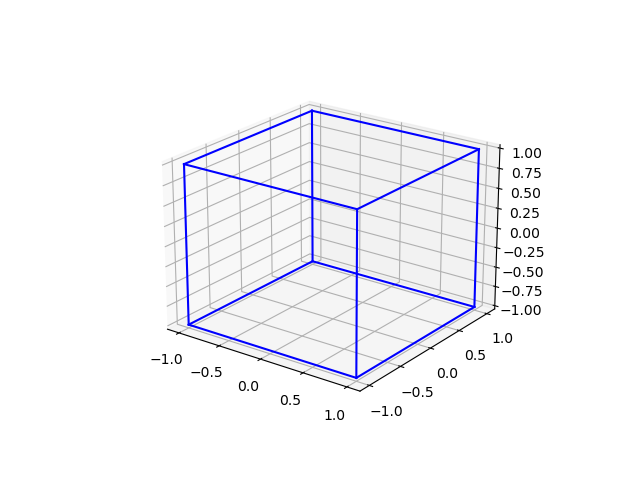
\includegraphics[width=15cm]{cube_1.png}
\end{center}
\caption{Cube 3D}
\end{figure}
\emph{2D Rotation Script}:\\
Steps:
\begin{enumerate}
\item Define the original square (4 points).
\item Apply a 2D rotation matrix to each point.
\item Plot the original and rotated squares.
\end{enumerate}
\emph{3D Rotation Script}:\\
Steps:
\begin{enumerate}
\item Define the original cube (8 points and edges).
\item Apply a 3D rotation matrix to each point.
\item Plot the original and rotated cubes.
\end{enumerate}
We'll use gnuplot's ability to plot lines and polygons.\\
\emph{Rotation Matrices Using Direction Cosines}\\
\emph{2D Rotation}\\
For rotation by angle \(\theta\) (counterclockwise):
\[
\begin{bmatrix}
x' \\ y'
\end{bmatrix}
=
\begin{bmatrix}
\cos\theta & -\sin\theta \\
\sin\theta & \cos\theta
\end{bmatrix}
\begin{bmatrix}
x \\ y
\end{bmatrix}.
\]
\emph{3D Rotation}\\
For rotation about an axis defined by unit vector \(\mathbf{u} = (l, m, n)\), the rotation
matrix \(R\) (Rodrigues' formula) is:
\[
R = I + (\sin\theta) K + (1 - \cos\theta) K^2,
\]
where \(K = \begin{bmatrix} 0 & -n & m \\ n & 0 & -l \\ -m & l & 0 \end{bmatrix}\).
\clearpage
\subsubsection{Scripts for Visualization}
\emph{1. 2D Rotation (Square)}\\
```gnuplot
\begin{verbatim}
set term png size 800,400
set output "2d_rotation.png"
set multiplot layout 1,2

# Original square
set title "Before Rotation"
set xrange [-2:2]
set yrange [-2:2]
set xlabel 'X Axes'
set ylabel 'Y Axes'
set size ratio 1
plot '-' with lines title "Square"
1 1
1 -1
-1 -1
-1 1
1 1
e

# Rotated square (45 degrees)
set title "After Rotation (45°)"
theta = pi/4
s = sin(theta)
c = cos(theta)
plot '-' using (c*$1 - s*$2):(s*$1 + c*$2) with lines title "Rotated Square"
1 1
1 -1
-1 -1
-1 1
1 1
e

unset multiplot
\end{verbatim}
```\\
\begin{figure}[!ht]
\begin{center}
 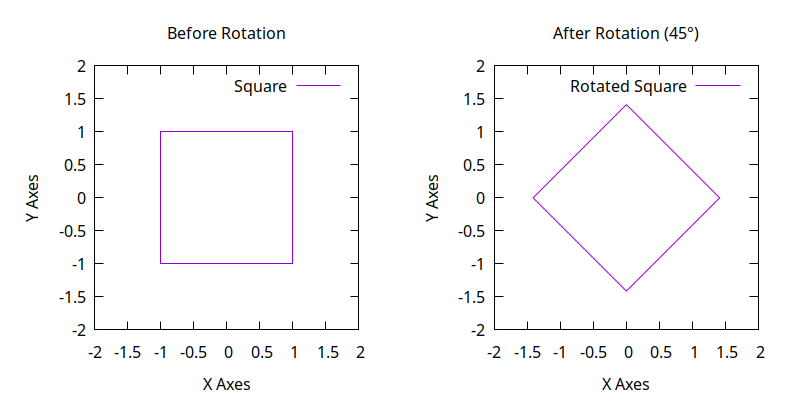
\includegraphics[width=15cm]{2d_rotation.png}
\end{center}
\caption{2D Rotation of a square}
\end{figure}
\emph{Explanation}:
\begin{itemize}
\item Plots a square before and after a 45° rotation.
\item The transformation is applied using the 2D rotation matrix.
\end{itemize}
\clearpage
\subsubsection{2D examples}
We created a c program that takes an angle in input from the user and automatically plots both the initial
and the rotated figures.\\
C
\begin{verbatim}
/* This program plots a square on the X,Y plane with edge 1 parallel to the axes
 and then plots the same square rotated by an angle theta given in input by the user
 */
#include <stdio.h>
#include <stdlib.h>
#define PI 3.141593
int main(int argc, char **argv){
  float theta,rtheta;
  char *gpfile;
  char *datafile;
  FILE *gpp,*dfp;
  if (argc < 2){
    fprintf(stderr, "usage:%s <angle (deg)>\n", argv[0]);
    return 1;
  }
  theta = atof(argv[1]); rtheta = PI*theta/180;
  gpfile = "rotated_square.gp";
  datafile = "square.dat";
  /* write the gnuplot script file */
  gpp = fopen(gpfile, "w\n");
    fprintf(gpp,"set terminal wxt persist\n");
    fprintf(gpp,"#set term pngcairo size 800,400\n");
    fprintf(gpp,"#set output '2d_rotation.png'\n");
    fprintf(gpp,"set multiplot layout 1,2\n");
    fprintf(gpp,"# Original square\n");
    fprintf(gpp,"set title 'Before Rotation'\n");
    fprintf(gpp,"set xrange [-2:2]\n");
    fprintf(gpp,"set yrange [-2:2]\n");
    fprintf(gpp,"set xlabel 'X Axes'\n");
    fprintf(gpp,"set ylabel 'Y Axes'\n");
    fprintf(gpp,"set size ratio 1\n");
    fprintf(gpp,"plot 'square.dat' with lines title 'Square', \\\n");
    fprintf(gpp,"'square.dat' with labels notitle offset 0.6,0.5 \n");
    fprintf(gpp,"set title 'After Rotation (%.1f°)'\n", theta);
    fprintf(gpp,"theta = %f\n", rtheta);
    fprintf(gpp,"s = sin(theta)\n");
    fprintf(gpp,"c = cos(theta)\n");
    fprintf(gpp,"plot 'square.dat' using (c*$1 - s*$2):(s*$1 + c*$2) \
    with lines title 'Rotated Square', \\\n");
    fprintf(gpp,"'square.dat'using (c*$1 - s*$2):(s*$1 + c*$2):3 \
    with labels offset 0.6,0.5 notitle\n");
  fclose(gpp);
    /* write the points data file */
  dfp = fopen(datafile, "w\n");
    fprintf(dfp," 1  1 A\n");
    fprintf(dfp," 1 -1 B\n");
    fprintf(dfp,"-1 -1 C\n");
    fprintf(dfp,"-1  1 D\n");
    fprintf(dfp," 1  1\n");
  fclose(dfp);
  /* run the script */
  system("gnuplot rotated_square.gp\n");
  return 0;
}
\end{verbatim}
The figure \ref{squarein} has been created with the following commands:\\
Bash
\begin{verbatim}
#To compile:
gcc rotated_square.c -o rotated_square
#To run
./rotated_square 15
\end{verbatim}
\begin{figure}[!ht]
\begin{center}
 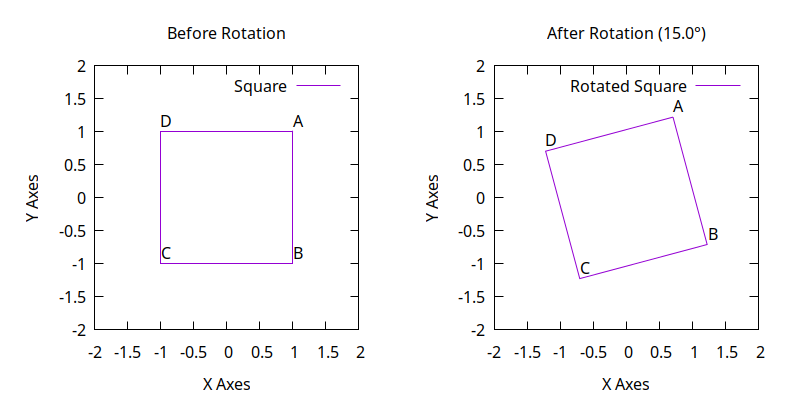
\includegraphics[width=15cm]{2d_rotation_input.png}
\end{center}
\caption{Square 2D Rotated of a given angle}
\label{squarein}
\end{figure}
\begin{figure}[!ht]
\begin{center}
 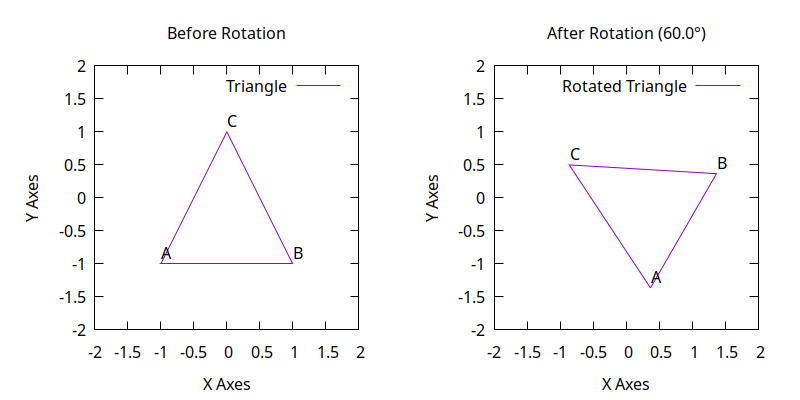
\includegraphics[width=15cm]{2d_rotated_triangle.png}
\end{center}
\caption{Triangle 2D Rotated of a given angle}
\label{trianglein}
\end{figure}
\subsubsection{3D examples}
\emph{2. 3D Rotation (Cube)}\\
\emph{Script}:\\
```gnuplot\\
\begin{verbatim}
# Set terminal and output
set terminal pngcairo enhanced font "Arial,12" size 1200,600
set output "3d_rotation.png"

# Set margins to create space between plots
set multiplot layout 1,2 spacing 20

# Common settings
set xyplane at 0
set view 60, 45, 1.2, 1
set border 4095
set ticslevel 0
set hidden3d
set view equal xyz
# Define rotation function (45 degrees around z and x axes)
theta = 45 * pi/180  # 45 degrees in radians

# First plot: Original cube
set title "Original Cube" offset 0,-1
set xlabel "X Axis" offset 0,1
set ylabel "Y Axis" offset 0,1
set zlabel "Z Axis" rotate by 90 offset -1,0
splot 'cube.dat' using 1:2:3 with lines title "" lw 2

# Second plot: Rotated cube
set title "Cube Rotated 45° around Z and X axes" offset 0,-1
set xlabel "X Axis" offset 0,1
set ylabel "Y Axis" offset 0,1
set zlabel "Z Axis" rotate by 90 offset -1,0
splot 'cube.dat' using ($1*cos(theta) - $2*sin(theta)):($1*sin(theta) + \
$2*cos(theta)):($3) with lines title "" lw 2

unset multiplot

# Alternative view with different rotation
set output "3d_rotation_alternative.png"
set multiplot layout 1,2 spacing 20

# First plot: Original cube
set title "Original Cube" offset 0,-1
set xlabel "X Axis" offset 0,1
set ylabel "Y Axis" offset 0,1
set zlabel "Z Axis" rotate by 90 offset -1,0
splot 'cube.dat' using 1:2:3 with lines title "" lw 2

# Second plot: Rotated cube (different angle)
theta2 = 60 * pi/180  # 60 degrees in radians
set title "Cube Rotated 60° around Z Axis" offset 0,-1
set xlabel "X Axis" offset 0,1
set ylabel "Y Axis" offset 0,1
set zlabel "Z Axis" rotate by 90 offset -1,0
splot 'cube.dat' using ($1*cos(theta2) - $2*sin(theta2)):($1*sin(theta2) + \
$2*cos(theta2)):3 with lines title "" lw 2

unset multiplot
\end{verbatim}
```\\
\emph{Data File} (\verb|`cube.dat`|):\\
```\\
\begin{verbatim}
1 1 1
1 -1 1
-1 -1 1
-1 1 1
1 1 1

1 1 -1
1 -1 -1
-1 -1 -1
-1 1 -1
1 1 -1

1 1 1
1 1 -1

1 -1 1
1 -1 -1

-1 -1 1
-1 -1 -1

-1 1 1
-1 1 -1
\end{verbatim}
```\\
\begin{figure}[!ht]
\begin{center}
 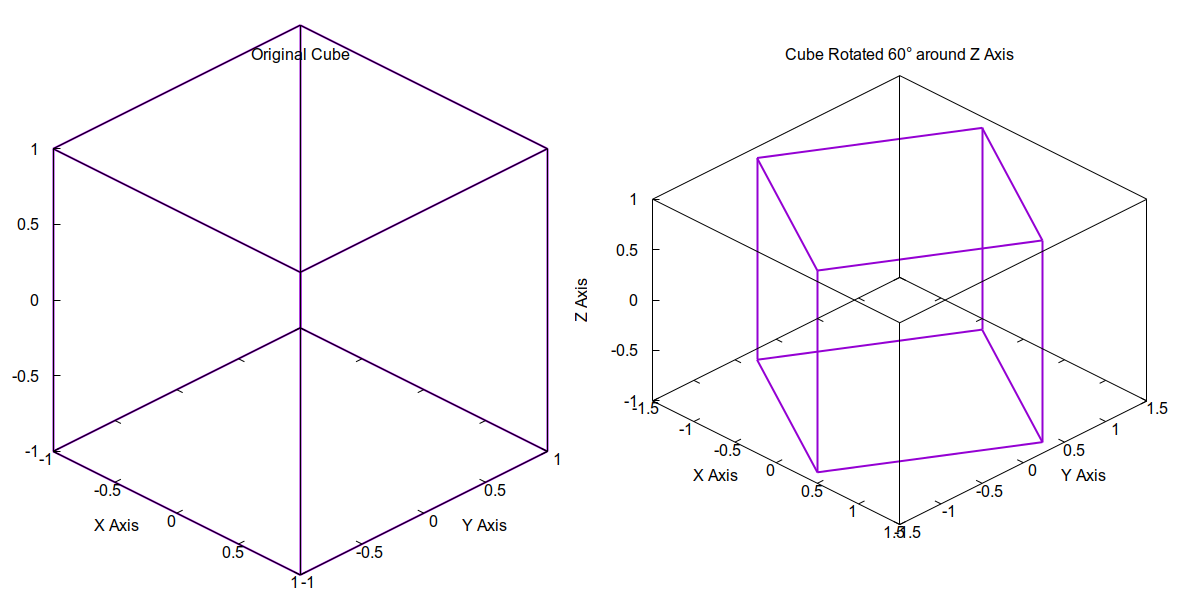
\includegraphics[width=15cm]{3d_rotation_alternative.png}
\end{center}
\caption{3D Rotation of a cube}
\end{figure}
\emph{Explanation}:
\begin{itemize}
\item Plots a cube before and after a 60° rotation about the z-axis.
\item The transformation uses the 3D rotation matrix for the z-axis.
\end{itemize}
\emph{Running the Scripts}
\begin{enumerate}
\item Save the scripts as `.plt` files and the cube data as `cube.dat`.
\item Run with:
   ```bash\\
\begin{verbatim}
   gnuplot 2d_rotation.plt
   gnuplot 3d_rotation.plt
\end{verbatim}
   ```\\
\item Outputs: \verb|`2d_rotation.png` and `3d_rotation.png`|.\\
 Let's consider an edge of the cube that originally was parallel to the X axis. For example, a vector along the X axis: (1, 0, 0).\\
 After rotation by $\theta$=60°, this vector becomes:
 \[
\begin{cases}
   x' = 1 \cdot \cos(60^{\circ}) - 0 \cdot \sin(60^{\circ}) = \cos(60^{\circ}) = 0.5\\
   y' = 1 \cdot \sin(60^{\circ}) + 0 \cdot \cos(60^{\circ}) = \sin(60^{\circ}) \approx 0.866\\
   z' = 0
\end{cases}
 \]
So the projected vector on the XY plane is (0.5, 0.866). The angle of this vector with the X-axis (which is (1,0)) is given by \(arctan(y'/x') = arctan(0.866/0.5) = arctan(1.732) \approx 60^{\circ}\).\\
Similarly, the angle with the Y-axis: the Y-axis is (0,1). The angle between the rotated vector and the Y-axis can be found by taking the dot product:\\
\(   (0.5, 0.866) \cdot (0,1) = 0.866 \)\\
The magnitude of the rotated vector is \( \sqrt(0.5^2+0.866^2)=1\), and the magnitude of the Y-axis vector is 1.\\
So the angle is \(\arccos(0.866) \approx 30^{\circ}\).\\
Therefore, yes, the edge that was originally along the X-axis, after a 60° rotation around Z, makes an angle of 60° with the X-axis and 30° with the Y-axis.\\
However, note that the cube has edges along the X, Y, and Z directions. The edges that were originally along the X and Y axes will rotate by 60° in the XY plane. The edges that were along the Z axis remain unchanged in direction (still parallel to Z).\\
So, in the second plot (60° rotation around Z), the projections of the edges that were originally along the X and Y axes will now be at 60° and 30° relative to the X and Y axes, respectively, as explained.
But note: the cube has multiple edges. The edge that was along the X axis will now be at 60° to the X-axis and 30° to the Y-axis. The edge that was along the Y axis will be rotated by 60° as well. Let's check the Y-axis edge:\\
Original vector along Y: (0,1,0)\\
After rotation:
\[
\begin{cases}
x' = 0\cdot \cos(60^{\circ}) - 1\cdot \sin(60^{\circ}) = -\sin(60^{\circ}) \approx -0.866\\
y' = 0\cdot \sin(60^{\circ}) + 1\cdot \cos(60^{\circ}) =  \cos(60^{\circ}) = 0.5
\end{cases}
\]
So the vector is (-0.866, 0.5). The angle with the X-axis: arctan(0.5/0.866) but note the negative x, so it's in the second quadrant. The angle from the positive X-axis is 180-30=150°. The angle with the Y-axis: the Y-axis is (0,1). The dot product: $(-0.866,0.5)\cdot(0,1)=0.5$, so the angle is arccos(0.5)=60°. So the edge that was along the Y-axis now makes 60° with the Y-axis and 150° with the X-axis.\\
So, in summary, for the 60° rotation around Z:
\begin{itemize}
\item The edge that was along X: makes 60° with X and 30° with Y.
\item  The edge that was along Y: makes 60° with Y and 150° with X (which is 30° with the negative X-axis).
\end{itemize}
 The script's second plot shows the cube after this rotation. The angles we see between the projected edges and the axes should be as calculated.
 However, note that the plot is a 3D plot with a particular view (60,45,1.2,1) and equal axes. The perspective might affect how we perceive the angles, but the projection of the edges onto the XY plane (if we look from above, i.e., along the Z-axis) would show these angles. But the plot is not necessarily from above; it's from an angle of 60° above the XY plane and 45° rotation in the plane. So the apparent angles in the plot might be distorted by the perspective.\\
But the question is about the projection on the XY plane. In the 3D plot, the axes are drawn in 3D and the cube is drawn in 3D. The projection of the cube's edges on the XY plane is not explicitly drawn, but we can imagine it by ignoring the Z-coordinate. However, the plot is a 3D plot, so the lines are drawn in 3D and the perspective projection is applied. Therefore, the angles we see on the screen are not the same as the true angles in the XY plane because of the 3D view.\\
If we want to see the true angles in the XY plane, we should set the view to look directly down the Z-axis: set view 0,0,1,1. But in the script, the view is set to 60,45,1.2,1.\\
So, to answer the question: Yes, the true projection of the rotated edge (originally along X) on the XY plane makes 60° with the X-axis and 30° with the Y-axis. But in the 3D plot with the given view, the apparent angles might be different due to perspective.\\
If you want to verify the angles, you might want to change the view to a top-down view (set view 0,0) for one of the plots.\\
Let me adjust the script to create two additional plots with a top-down view to clearly show the XY plane projection.\\
We'll create a new file for the top-down view.\\
Alternatively, we can add a third multiplot to the same script to show the top-down view.\\
But note: the user's question is about the existing script. We are just explaining the angles.\\
Since the user is asking about the script they provided, we can confirm that the calculation is correct and the angles in the XY plane are 60° and 30° as described.\\
However, if the user wants to see the true angles, they might need to change the view.\\
Let me modify the script to include a top-down view for the 60° rotation.
We'll create a new output file and set the view to 0,0 (top-down).\\
But note: the original script already produces two multiplots. We are going to add a third one? Or replace the second one?\\
Since the user might want to see both, we can create an additional multiplot with top-down view.\\
Let's do:
\begin{itemize}
\item First multiplot: original and 60° rotation with the same 3D view as before.
\item Second multiplot: top-down view of the original and 60° rotation.
\end{itemize}
 We'll change the script as follows:\\
 ... [keep the first two multiplots] ...\\
 Then:
\begin{verbatim}
set output "3d_rotation_topdown.png"
set multiplot layout 1,2 spacing 20

set view 0,0  # Top-down view, along Z-axis

# First plot: Original cube (top-down)
set title "Original Cube (Top-Down View)" offset 0,-1
set xlabel "X Axis" offset 0,1
set ylabel "Y Axis" offset 0,1
set zlabel "Z Axis" rotate by 90 offset -1,0
# Since we are looking along Z, the Z coordinate will be ignored in the projection,
#but the plot is still 3D.
splot 'cube.dat' using 1:2:3 with lines title "" lw 2

# Second plot: Rotated cube (top-down)
set title "Cube Rotated 60° around Z Axis (Top-Down)" offset 0,-1
set xlabel "X Axis" offset 0,1
set ylabel "Y Axis" offset 0,1
set zlabel "Z Axis" rotate by 90 offset -1,0
splot 'cube.dat' using ($1*cos(theta2) - $2*sin(theta2)):($1*sin(theta2) \
+ $2*cos(theta2)):3 with lines title "" lw 2

unset multiplot
\end{verbatim}
But note: in top-down view, the Z coordinate is ignored because we are looking from Z infinity. So the plot is effectively a 2D projection. The cube's edges that are parallel to Z will appear as points (if the cube is drawn with lines, the vertical lines will be points). But the cube data file 'cube.dat' probably has the edges of the cube. If it is drawn with lines, the vertical lines will be drawn as points because the Z coordinate is the same for the top and bottom? Actually, the cube data file should have the 12 edges of the cube. In top-down view, the top and bottom faces will overlap, and the vertical edges will be points.\\
Alternatively, we can plot only the top face or bottom face to avoid confusion.\\
But let's assume the cube data file is standard and drawn with lines. The top-down view will show the XY projection. This will clearly show the rotation angle in the XY plane.
In the script, the 60° rotation is applied \emph{only around the Z-axis} using this transformation:\\
```\\
gnuplot\\
\verb|($1*cos(theta2) - $2*sin(theta2)):($1*sin(theta2) + $2*cos(theta2)):3|
```\\
This is a rotation matrix for rotation around the Z-axis by angle $\theta$:\\
\[
\begin{bmatrix}
 \cos \theta&  -\sin\theta&  0\\
 \sin \theta&   \cos\theta&  0\\
  0         &     0       &  1\\
\end{bmatrix}
\]
For \(\theta = 60^{\circ}\):
\begin{itemize}
\item An edge originally aligned with the X-axis will rotate to make a 60° angle with the X-axis
\item The same edge will make a 30° angle with the Y-axis (since 90° - 60° = 30°)
\end{itemize}
However, there's a \emph{key point} about the visualization: In a 3D perspective view, the apparent angles you see on the 2D screen are affected by:
\begin{enumerate}
\item The 3D perspective (`set view 60, 45, 1.2, 1`)
\item The fact that we're looking at the cube from an angle, not straight down the Z-axis
\end{enumerate}
So while mathematically the projection onto the XY-plane has the 60°/30° relationship you described, the perspective distortion in the 3D view might make these angles appear different on screen.
If you want to see the true XY-plane projection angles, you could add a third view with:
```gnuplot\\
\verb|set view 0, 0  # Look straight down the Z-axis|\\
```\\
This would show the pure 2D projection where the angles would be exactly 60° and 30° as calculated.
\end{enumerate}
This demonstrates how direction cosines underpin rotation matrices and their visual effects in
2D/3D spaces.
\subsection{Rotation along all 3 axes}
We will visualize a 3D cube and its rotation around all three axes (x, y, z).\\
The rotation will be defined by a rotation matrix that combines rotations around each axis.
We'll use the following rotation matrices:
\[
\begin{cases}
   R_x(\alpha) = [1, 0, 0; 0, \cos(\alpha), -\sin(\alpha); 0, \sin(\alpha), \cos(\alpha)]\\
   R_y(\beta) = [\cos(\beta), 0, \sin(\beta); 0, 1, 0; -\sin(\beta), 0, cos(\beta)]\\
   R_z(\gamma) = [\cos(\gamma), -\sin(\gamma), 0; \sin(\gamma), \cos(\gamma), 0; 0, 0, 1]\\
\end{cases}
\]
The combined rotation matrix \(R = R_z(\gamma) * R_y(\beta) * R_x(\alpha) \) (applied in order: x, then y, then z).
However, note: the order of multiplication matters. We'll define the rotation as:
\[
\begin{matrix}
 [x']\\
 [y']\\
 [z']\\
\end{matrix}
=
\begin{matrix}
[\cos(\gamma)\; -\sin(\gamma)\; 0]& [\cos(\beta)\;  0\;\;  \sin(\beta)]& [1\;\;     0\;\;      0   ]\\
[\sin(\gamma)\;  \cos(\gamma)\; 0]& [0\;       1\;     0   ]& [0\;\;  \cos(\alpha)\; -\sin(\alpha)]\\
[0 \;\;      0\;\;      1]& [-\sin(\beta) 0\;  \cos(\beta)]& [0\;\;  \sin(\alpha)\;  \cos(\alpha)]\\
\end{matrix}
\begin{matrix}
[x]\\
[y]\\
[z]\\
\end{matrix}
\]
We can break it down step by step, in gnuplot we can apply the matrix multiplication by breaking into steps or precomputing the combined matrix.\\
Alternatively, we can apply the rotations in the following order (which is common in aerospace, for example, using Euler angles):\\
First rotate around x-axis by \( \alpha\), then around y-axis by \(\beta\), then around z-axis by \(\gamma\).
Let's define:
\begin{verbatim}
   alpha = rotation around x-axis (in radians)
   beta  = rotation around y-axis (in radians)
   gamma = rotation around z-axis (in radians)
\end{verbatim}
We will create a function for the rotated coordinates:
{
\tiny
\begin{verbatim}
   x_rot = cos(gamma)*cos(beta)*x + (cos(gamma)*sin(beta)*sin(alpha) - sin(gamma)*cos(alpha))*y + (cos(gamma)*sin(beta)*cos(alpha) + sin(gamma)*sin(alpha))*z
   y_rot = sin(gamma)*cos(beta)*x + (sin(gamma)*sin(beta)*sin(alpha) + cos(gamma)*cos(alpha))*y + (sin(gamma)*sin(beta)*cos(alpha) - cos(gamma)*sin(alpha))*z
   z_rot = -sin(beta)*x + cos(beta)*sin(alpha)*y + cos(beta)*cos(alpha)*z
\end{verbatim}
}
Note: the above is the combined rotation matrix for the order: x, then y, then z.\\
Here is shown step by step:\\
\begin{itemize}
\item Step 1: Rotate around x by alpha:
\begin{verbatim}
   x1 = x
   y1 = y*cos(alpha) - z*sin(alpha)
   z1 = y*sin(alpha) + z*cos(alpha)
\end{verbatim}
\item Step 2: Rotate around y by beta:
\begin{verbatim}
   x2 = x1*cos(beta) + z1*sin(beta)
   y2 = y1
   z2 = -x1*sin(beta) + z1*cos(beta)
\end{verbatim}
\item Step 3: Rotate around z by gamma:
\begin{verbatim}
   x3 = x2*cos(gamma) - y2*sin(gamma)
   y3 = x2*sin(gamma) + y2*cos(gamma)
   z3 = z2
\end{verbatim}
\end{itemize}
So we can write the transformation in gnuplot as:
{
\scriptsize
\begin{verbatim}
   x_rot = (x*cos(beta) + (y*sin(alpha) + z*cos(alpha))*sin(beta)) * cos(gamma) - (y*cos(alpha) - z*sin(alpha)) * sin(gamma)
   y_rot = (x*cos(beta) + (y*sin(alpha) + z*cos(alpha))*sin(beta)) * sin(gamma) + (y*cos(alpha) - z*sin(alpha)) * cos(gamma)
   z_rot = -x*sin(beta) + (y*sin(alpha) + z*cos(alpha))*cos(beta)
\end{verbatim}
}
Let's set some example angles, say 45 degrees around each axis.\\
Note: the above is one common order (Z-Y-X). There are multiple conventions. We'll stick with this.
We'll create a data file for a cube. The cube data file 'cube.dat' should contain the coordinates of the cube's edges.\\
Let's generate the cube data. The cube has 8 vertices and we'll draw 12 edges.\\
Let's assume we have a file 'cube.dat' that has the data in the format:
\begin{verbatim}
   x1 y1 z1
   x2 y2 z2
   ...
\end{verbatim}
 and we use `with lines` to connect the points. We need to define the edges appropriately.
 We can create a cube with vertices at \((\pm1, \pm1, \pm1)\). We'll list the edges in order.
\begin{verbatim}
   -1 -1 -1
    1 -1 -1
    1  1 -1
   -1  1 -1
   -1 -1 -1  (close the bottom face)

   -1 -1  1
    1 -1  1
    1  1  1
   -1  1  1
   -1 -1  1  (close the top face)

   Then draw the vertical edges:
   -1 -1 -1
   -1 -1  1

    1 -1 -1
    1 -1  1

    1  1 -1
    1  1  1

   -1  1 -1
   -1  1  1
\end{verbatim}
Note: the data must be separated by blank lines to break the lines.
Gnuplot requires one blank line to separate data blocks.
We are going to use the following structure for the 'cube.dat':
\begin{verbatim}
   # bottom face
   -1 -1 -1
    1 -1 -1
    1  1 -1
   -1  1 -1
   -1 -1 -1

   # top face
   -1 -1  1
    1 -1  1
    1  1  1
   -1  1  1
   -1 -1  1

   # vertical edges
   -1 -1 -1
   -1 -1  1

    1 -1 -1
    1 -1  1

    1  1 -1
    1  1  1

   -1  1 -1
   -1  1  1
\end{verbatim}
 And we separate each block (face and each edge) by a blank line.
 Now, we'll write the gnuplot script.\\
 Steps:
\begin{enumerate}
\item Set terminal and output.
\item Set multiplot to show original and rotated cube side by side.
\item Define the rotation angles (in degrees, then convert to radians).
\item For the rotated cube, apply the rotation to each point.
\end{enumerate}
Let's set:
\begin{verbatim}
   alpha = 45  # around x
   beta  = 45  # around y
   gamma = 45  # around z
\end{verbatim}
But note: 45 degrees in radians is \(\pi/4\).\\
We'll define:
\begin{verbatim}
   a = alpha * pi/180
   b = beta * pi/180
   c = gamma * pi/180
\end{verbatim}
Then use the formulas:\\
{
\scriptsize
\begin{verbatim}
   x_rot = (x*cos(b) + (y*sin(a) + z*cos(a))*sin(b)) * cos(c) - (y*cos(a) - z*sin(a)) * sin(c)
   y_rot = (x*cos(b) + (y*sin(a) + z*cos(a))*sin(b)) * sin(c) + (y*cos(a) - z*sin(a)) * cos(c)
   z_rot = -x*sin(b) + (y*sin(a) + z*cos(a))*cos(b)
\end{verbatim}
}
We'll plot the original cube and the rotated cube.
Here an example of 3D rotation with rotation matrices and modify the gnuplot script accordingly, using a comprehensive approach:\\
\emph{Rotation Matrices for 3D Rotation}\\
The rotation matrices around each axis are:\\
\emph{Rotation around X-axis} ($\alpha$):\\
\[
R_x(\alpha)
=
\begin{bmatrix}
         1   &          0 &         0     \\
         0   &\cos(\alpha)&  -\sin(\alpha)\\
         0   &\sin(\alpha)&   \cos(\alpha)\\
\end{bmatrix}
\]
\emph{Rotation around Y-axis} (\(\beta\)):\\
\[
R_y(\beta)
=
\begin{bmatrix}
         \cos(\beta) &   0 &   \sin(\beta)\\
              0      &   1 &          0   \\
         -\sin(\beta)&   0 &   \cos(\beta)\\
\end{bmatrix}
\]
\emph{Rotation around Z-axis} (\(\gamma\)):\\
\[
R_z(\gamma)
=
\begin{bmatrix}
         \cos(\gamma)&   -\sin(\gamma)&   0\\
         \sin(\gamma)&    \cos(\gamma)&   0\\
             0       &          0     &   1\\
\end{bmatrix}
\]
\emph{Modified Gnuplot Script}\\
```gnuplot
{
\scriptsize
\begin{verbatim}
# Set terminal and output
set terminal pngcairo enhanced font "Arial,12" size 1600,800
set output "3d_rotation_complete.png"
# Set margins and layout
set multiplot layout 2,2 spacing 20
# Common settings
set xyplane at 0
set view 60, 30, 1.2, 1
set border 4095
set ticslevel 0
set hidden3d
set view equal xyz
# Define rotation angles (in degrees)
alpha = 30 * pi/180  # 30 degrees around X-axis
beta = 45 * pi/180   # 45 degrees around Y-axis
gamma = 60 * pi/180  # 60 degrees around Z-axis
# First plot: Original cube
set title "Original Cube" offset 0,-1
set xlabel "X Axis" offset 0,1
set ylabel "Y Axis" offset 0,1
set zlabel "Z Axis" rotate by 90 offset -1,0
splot 'cube.dat' using 1:2:3 with lines title "" lw 2
# Second plot: Rotated around X-axis
set title "Rotation around X-axis (\alpha=30°)" offset 0,-1
splot 'cube.dat' using 1:($2*cos(alpha) - $3*sin(alpha)):($2*sin(alpha) \
+ $3*cos(alpha)) with lines title "" lw 2
# Third plot: Rotated around Y-axis
set title "Rotation around Y-axis (\beta=45°)" offset 0,-1
splot 'cube.dat' using ($1*cos(beta) + $3*sin(beta)):2:(-$1*sin(beta) \
+ $3*cos(beta)) with lines title "" lw 2
# Fourth plot: Rotated around Z-axis
set title "Rotation around Z-axis (\gamma=60°)" offset 0,-1
splot 'cube.dat' using ($1*cos(gamma) - $2*sin(gamma)):($1*sin(gamma) \
+ $2*cos(gamma)):3 with lines title "" lw 2
unset multiplot
# Combined rotation plot
set terminal pngcairo enhanced font "Arial,12" size 1200,600
set output "3d_rotation_combined.png"
set multiplot layout 1,2 spacing 20
# Combined rotation (R_z * R_y * R_x)
set title "Original Cube" offset 0,-1
splot 'cube.dat' using 1:2:3 with lines title "" lw 2
set title "Combined Rotation (R_z(60°)·R_y(45°)·R_x(30°))" offset 0,-1
splot 'cube.dat' using \
(($1*cos(beta) + ($2*sin(alpha) + $3*cos(alpha))*sin(beta))*cos(gamma) - (($2*cos(alpha) -
$3*sin(alpha))*sin(gamma))) : \
(($1*cos(beta) + ($2*sin(alpha) + $3*cos(alpha))*sin(beta))*sin(gamma) + (($2*cos(alpha) -
$3*sin(alpha))*cos(gamma))) : \
(-$1*sin(beta) + ($2*sin(alpha) + $3*cos(alpha))*cos(beta)) \
with lines lw 2 notitle
unset multiplot
\end{verbatim}
}
```\\
\emph{Cube Data File} (`cube.dat`)\\
We use a file called `cube.dat` with the following content:\\
{
\scriptsize
\begin{verbatim}
# Cube vertices
-1 -1 -1
1 -1 -1
1 1 -1
-1 1 -1
-1 -1 -1

-1 -1 1
1 -1 1
1 1 1
-1 1 1
-1 -1 1

1 -1 -1
1 -1 1

1 1 -1
1 1 1

-1 1 -1
-1 1 1

-1 -1 -1
-1 -1 1
\end{verbatim}
}
\begin{figure}[!ht]
\begin{center}
 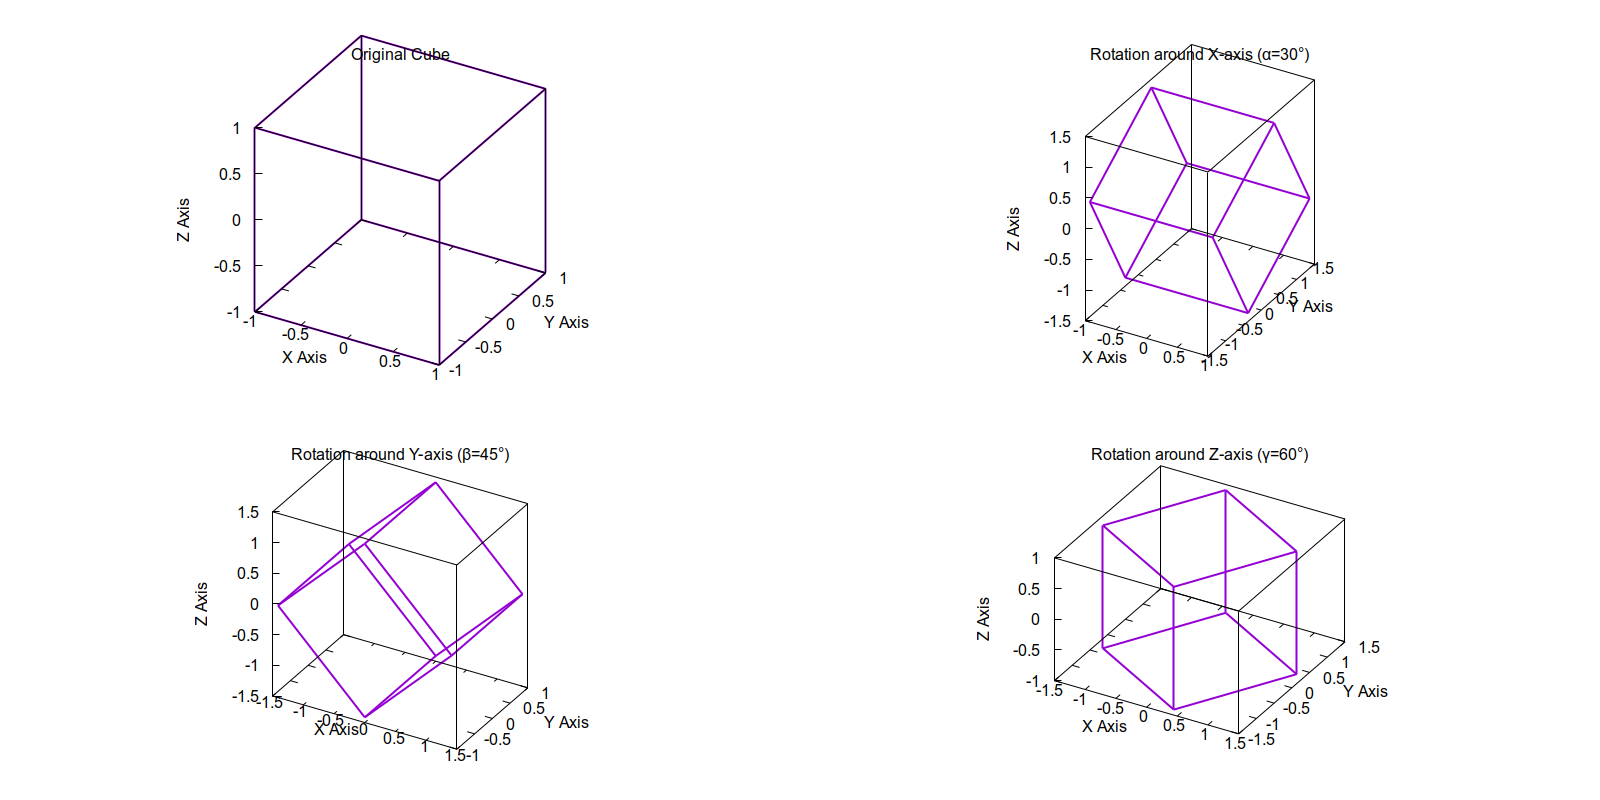
\includegraphics[width=18cm]{3d_rotation_complete.png}
\end{center}
\caption{3D Rotation of a cube along the 3 axes}
\label{splitcube}
\end{figure}
\clearpage
\emph{Alternative Script with Step-by-Step Visualization}\\
```gnuplot\\
\begin{verbatim}
# Step-by-step rotation visualization
set terminal pngcairo enhanced font "Arial,12" size 1600,1200
set output "3d_rotation_step_by_step.png"

set multiplot layout 3,3 spacing 15

# Define angles
alpha = 30 * pi/180
beta = 45 * pi/180
gamma = 60 * pi/180

# Row 1: X-axis rotation steps
set view 60, 30
set title "Original" offset 0,-1
splot 'cube.dat' using 1:2:3 with lines lw 2

set title "After R_x(30°)" offset 0,-1
splot 'cube.dat' using 1:($2*cos(alpha) - $3*sin(alpha)):($2*sin(alpha) \
+ $3*cos(alpha)) with lines lw 2

set title "After R_x(30°)·R_y(45°)" offset 0,-1
splot 'cube.dat' using \
($1*cos(beta) + ($2*sin(alpha) + $3*cos(alpha))*sin(beta)) : \
($2*cos(alpha) - $3*sin(alpha)) : \
(-$1*sin(beta) + ($2*sin(alpha) + $3*cos(alpha))*cos(beta)) \
with lines lw 2

# Row 2: Y-axis rotation steps
set title "Original" offset 0,-1
splot 'cube.dat' using 1:2:3 with lines lw 2

set title "After R_y(45°)" offset 0,-1
splot 'cube.dat' using ($1*cos(beta) + $3*sin(beta)):2:(-$1*sin(beta) \
+ $3*cos(beta)) with lines lw 2

set title "After R_y(45°)·R_z(60°)" offset 0,-1
splot 'cube.dat' using \
(($1*cos(beta) + $3*sin(beta))*cos(gamma) - $2*sin(gamma)) : \
(($1*cos(beta) + $3*sin(beta))*sin(gamma) + $2*cos(gamma)) : \
(-$1*sin(beta) + $3*cos(beta)) with lines lw 2

# Row 3: Z-axis rotation steps
set title "Original" offset 0,-1
splot 'cube.dat' using 1:2:3 with lines lw 2

set title "After R_z(60°)" offset 0,-1
splot 'cube.dat' using ($1*cos(gamma) - $2*sin(gamma)):($1*sin(gamma) \
+ $2*cos(gamma)):3 with lines lw 2

set title "After R_z(60°)·R_x(30°)" offset 0,-1
splot 'cube.dat' using \
($1*cos(gamma) - $2*sin(gamma)) : \
(($1*sin(gamma) + $2*cos(gamma))*cos(alpha) - $3*sin(alpha)) : \
(($1*sin(gamma) + $2*cos(gamma))*sin(alpha) + $3*cos(alpha)) \
with lines lw 2

unset multiplot
\end{verbatim}
```\\
\begin{figure}[!ht]
\begin{center}
 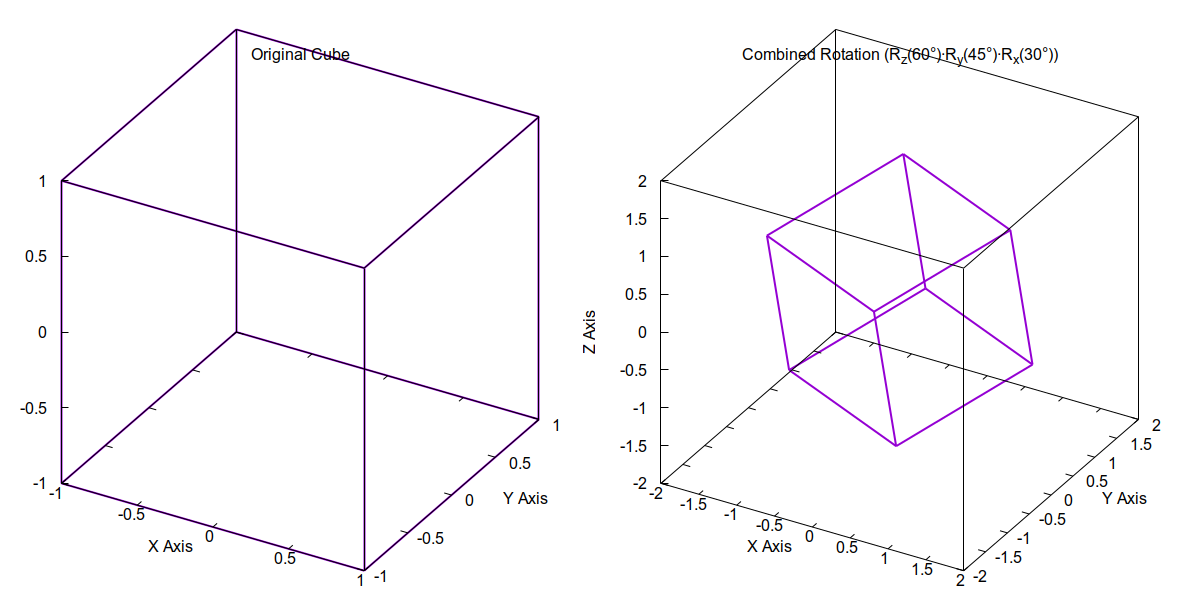
\includegraphics[width=15cm]{3d_rotation_combined.png}
\end{center}
\caption{Combined 3D Rotation of a cube}
\label{combcube}
\end{figure}
This script demonstrates:
\begin{enumerate}
\item \emph{Individual rotations} around each axis (X, Y, Z)
\item \emph{Combined rotations} showing the effect of applying multiple rotation matrices
\item \emph{Step-by-step visualization} showing how rotations accumulate
\end{enumerate}
The rotation matrices are applied in the order specified (note that matrix multiplication is not commutative, so order matters).
\subsection{Animation}
We are going to create a C program that uses the \verb|gnuplot_i| library to create an animation of 3D rotations.
The idea is to rotate a cube step by step around each of the three axes (X, Y, Z) and then a combined rotation.
We will break down the rotation into small steps (e.g., 5° or 10° per step) and update the plot in a loop.\\
Steps:
\begin{enumerate}
\item Include the necessary headers and the \verb|gnuplot_i| library.
\item Define the cube data (the same as in cube.dat) in the program or read from file.
\item Initialize gnuplot.
\item Set up the terminal (maybe for gif animation or just for on-screen display).
\item For each step in the rotation, compute the new coordinates of the cube and plot them.
\item We'll do three separate rotations (X, Y, Z) and then a combined rotation.
\end{enumerate}
However, note that the provided gnuplot script does multiple plots in one image (multiplot).
But for animation, we want to show one rotation at a time, and then the combined, in sequence.
We can structure the animation as follows:
\begin{enumerate}
\item Original cube.
\item Rotation around X-axis from 0 to 30° in steps\\(e.g., 30° total, step 5° \(\rightarrow\) 6 steps).
\item Rotation around Y-axis from 0 to 45° in steps.
\item Rotation around Z-axis from 0 to 60° in steps.
\item Combined rotation (all three) in steps.
\end{enumerate}
Since the example script uses 30,45,60, we can do:
\begin{itemize}
\item For X-axis: 0 to 30° in steps of 5° (or 10°)
\item For Y-axis: 0 to 45° in steps
\item For Z-axis: 0 to 60° in steps
\item Then combined: apply all three rotations in the same step increments.
\end{itemize}
Note: the combined rotation in the script is \verb|R_z * R_y * R_x| (applied in that order).
We can break the combined rotation into the same number of steps as the maximum of the steps for each rotation.
However, to keep it simple, we can do:\\
Let steps = 30 (for example) and then for each step i from 0 to steps:\\
\begin{verbatim}
        alpha = (30.0 * i / steps) * pi/180
        beta  = (45.0 * i / steps) * pi/180
        gamma = (60.0 * i / steps) * pi/180
\end{verbatim}
Then for each step, we compute the cube rotated by (alpha, beta, gamma) in the order: X, then Y, then Z.\\
Note: the script does the combined rotation as Z * Y * X (matrix multiplication order). We can compute the rotated points as:\\
{
\scriptsize
\begin{verbatim}
   [x']   [cos(gamma)  -sin(gamma)  0]   [cos(beta)  0  sin(beta)]   [1     0          0       ]   [x]
   [y'] = [sin(gamma)   cos(gamma)  0] * [0          1  0        ] * [0  cos(alpha) -sin(alpha)] * [y]
   [z']   [0           0           1 ]   [-sin(beta) 0  cos(beta)]   [0  sin(alpha)  cos(alpha)]   [z]
\end{verbatim}
}

We can break it down step by step for the animation:\\
Step 1: Rotate the cube around X by alpha, then around Y by beta, then around Z by gamma.\\
Note: the matrix multiplication is applied from right to left. So we can compute:\\

\begin{verbatim}
   First, apply X rotation:
        x1 = x
        y1 = y*cos(alpha) - z*sin(alpha)
        z1 = y*sin(alpha) + z*cos(alpha)

   Then, apply Y rotation to (x1, y1, z1):
        x2 = x1*cos(beta) + z1*sin(beta)
        y2 = y1
        z2 = -x1*sin(beta) + z1*cos(beta)

   Then, apply Z rotation to (x2, y2, z2):
        x3 = x2*cos(gamma) - y2*sin(gamma)
        y3 = x2*sin(gamma) + y2*cos(gamma)
        z3 = z2
\end{verbatim}
So the combined transformation is:\\
{
\scriptsize
\begin{verbatim}
x3 = (x*cos(beta) + (y*sin(alpha)+z*cos(alpha))*sin(beta)) * cos(gamma) - (y*cos(alpha)-z*sin(alpha)) * sin(gamma)
y3 = (x*cos(beta) + (y*sin(alpha)+z*cos(alpha))*sin(beta)) * sin(gamma) + (y*cos(alpha)-z*sin(alpha)) * cos(gamma)
z3 = -x*sin(beta) + (y*sin(alpha)+z*cos(alpha)) * cos(beta)
\end{verbatim}
}
This is the same as the expression in the script.
We will create a function to compute the rotated point for a given (x,y,z) and angles (alpha, beta, gamma).
We'll also create a function to plot the cube given the set of points and the gnuplot handle.
for the animation we will:
\begin{enumerate}
\item Create a GIF animation by setting the terminal to gif and then outputting each frame.
\item display it on the screen in a window (like the \verb|gnuplot_i| example animation.c).
\end{enumerate}
Let's do:
\begin{quote}
        If a command line argument is given (e.g., "gif"), then set the terminal to gif and output to a file.
        Otherwise, use the default terminal (x11 or wxt) for on-screen display.
\end{quote}
We can use the gnuplot\_cmd to set the terminal and output accordingly.\\
Steps for the program:\\
\begin{enumerate}
\item Parse command line arguments to decide on output (gif or screen).
\item Define the cube points (we can hardcode the same as in cube.dat).
\item Initialize gnuplot.
\item If gif mode, set terminal to gif and set output file.
\item For each step i from 0 to N (N=number of steps, let's say 30):
\begin{itemize}
\item Compute alpha, beta, gamma for step i.
\item Compute the rotated cube points.
\item Plot the cube (with lines) and maybe also the original cube for reference?
\end{itemize}
 \item Close the gnuplot handle.
\end{enumerate}
The example script also shows the original cube and the individual rotations.
We might want to show four subplots (like the script) but that would require multiplot.
Note: the \verb|gnuplot_i| library does not directly support multiplot. We can send multiplot commands via \verb|gnuplot_cmd|.
Alternatively, we can do four separate plots for each step (like the script) but that would require 4 times the data.
Let's reconsider: the animation should show the rotation in a fluid way. Maybe we don't need the multiplot for animation.
We can do:
\begin{itemize}
\item First, show the original cube for a second.
\item Then, rotate around X axis from 0 to 30° (with the cube in the same plot).
\item Then, rotate around Y axis from 0 to 45° (starting from the cube that has been rotated by X 30°? or from the original?)
\item Then, rotate around Z axis from 0 to 60° (again, from the previous state? or from the original?)
\end{itemize}
The script does:
\begin{itemize}
\item First plot: original
\item Second: only X rotation
\item Third: only Y rotation (on the original cube, not on the X-rotated one)
\item Fourth: only Z rotation (on the original)
\end{itemize}
And then the combined: all three applied to the original.\\
So for the animation, we can do:
\begin{itemize}
\item Part 1: Original cube (static)
\item Part 2: Rotation around X (from 0 to 30) on the original cube.
\item Part 3: Rotation around Y (from 0 to 45) on the original cube.
\item Part 4: Rotation around Z (from 0 to 60) on the original cube.
\item Part 5: Combined rotation (from 0 to 30,0 to 45,0 to 60) on the original cube.
\end{itemize}
Note: the combined rotation is not the same as doing the three rotations one after the other on the cube, because each rotation is applied to the original, not cumulative.
Alternatively, we can do:
\begin{itemize}
\item Part 1: Original
\item Part 2: X rotation (0 to 30) on the original \(\rightarrow\) result A
\item Part 3: Y rotation (0 to 45) on result A \(\rightarrow\) result B
\item Part 4: Z rotation (0 to 60) on result B \(\rightarrow\) result C
\end{itemize}

That would be a cumulative rotation, which is different from the script.
Since the script does not do cumulative, but each rotation is independent, we'll do independent rotations.
However, the combined rotation in the script is applied as a single transformation \verb|(R_z * R_y * R_x)| to the original.
So we have two different things:
\begin{itemize}
\item Individual rotations: each is applied to the original.
\item Combined rotation: also applied to the original.
\end{itemize}
The animation for the combined rotation is not the same as the individual rotations applied sequentially.
We'll stick to the script's approach: each rotation is independent and applied to the original.
herefore, we can structure the animation as:\\
\begin{verbatim}
        Step 0: Show original cube.
        Then, for i in steps:
            Show:
                Original cube (maybe in one subplot)
                X-rotated cube (angle = alpha_i) in another subplot
                Y-rotated cube (angle = beta_i) in another subplot
                Z-rotated cube (angle = gamma_i) in another subplot
        Then, for the combined, we can do:
            For i in steps:
                Show the combined rotation
                (alpha_i, beta_i, gamma_i) in a single plot?
                or in the multiplot?
\end{verbatim}
But the script has two multiplots: one for the individual rotations and one for the combined.
We can do:\\
        First multiplot: 4 subplots (original, X, Y, Z) for each step i.\\
        Then, second multiplot: 2 subplots (original and combined) for each step i.\\
That would require 6 plots per step, which might be heavy and the animation might be slow.
Alternatively, we can break the animation into segments:
\begin{itemize}
\item Segment 1: Individual rotations (multiplot with 4 subplots) for steps i=0..N.
\item Segment 2: Combined rotation (multiplot with 2 subplots) for steps i=0..N.
\end{itemize}
Note: the combined rotation uses the same angles as the individual, so we can do:
\begin{verbatim}
        For each step i from 0 to N:
            Show the multiplot of individual rotations (original, X, Y, Z)
            and the combined (original and combined) in two separate frames?
\end{verbatim}
Actually, the script produces two images: one with the individual rotations and one with the combined.
We are going to produce an animation that shows:

\begin{verbatim}
        Frame 0: Original cube
        (all four subplots show the original?
        but then we rotate the other three)

        Then, for i=1 to N:
            In the second subplot, show the cube rotated by X (alpha_i)
            In the third subplot, show the cube rotated by Y (beta_i)
            In the fourth subplot, show the cube rotated by Z (gamma_i)

        Then, for the combined, we can do a separate animation:

            Frame 0: Original cube (in both subplots)
            Then, for i=1 to N:
                Left subplot: original cube
                Right subplot: cube rotated by (alpha_i, beta_i, gamma_i)
\end{verbatim}
So we'll create two animations:\\
\begin{itemize}
\item Animation 1: Individual rotations (4 subplots)
\item Animation 2: Combined rotation (2 subplots)
\end{itemize}
We can either combine them into one video (first animation1, then animation2) or make two separate files.
Let's do:
\begin{verbatim}
        If gif output is chosen, we'll create two gif files:
        one for individual and one for combined.

        If screen output, we'll show first the individual rotation animation
        and then the combined.
\end{verbatim}
Steps:
\begin{itemize}
\item Part 1: Individual rotations\\
            Set multiplot layout 2,2\\
            For each step i from 0 to N:
\begin{itemize}
       \item    Set the title for each subplot.
       \item    Plot the original cube in the first subplot.
       \item    Plot the X-rotated cube in the second subplot (angle = \verb|alpha_i|).
       \item    Plot the Y-rotated cube in the third subplot (angle = \verb|beta_i|).
       \item    Plot the Z-rotated cube in the fourth subplot (angle = \verb|gamma_i|).
\end{itemize}
            Unset multiplot.
\item Part 2: Combined rotation
            Set multiplot layout 1,2\\
            For each step i from 0 to N:
\begin{itemize}
       \item    Plot the original cube in the first subplot.
       \item    Plot the combined rotated cube in the second subplot (angles = \verb|alpha_i, beta_i, gamma_i|).
\end{itemize}
            Unset multiplot.
\end{itemize}
We need to send the multiplot commands via \verb|gnuplot_cmd|.\\
However, the \verb|gnuplot_i| library does not have a built-in function for multiplot. We have to send the commands as strings.
We can do:
\begin{verbatim}
        gnuplot_cmd(handle, "set multiplot layout 2,2");
        ... then for each subplot, we set the title and plot the data ...
\end{verbatim}
Note: when we use multiplot, we have to set the title and labels for each subplot individually.\\
We can set the title for each subplot by:
\begin{verbatim}
        gnuplot_cmd(handle, "set title 'Original Cube'");
        gnuplot_cmd(handle, "splot ...");
\end{verbatim}
but then the next plot will be in the next subplot.\\
However, the \verb|gnuplot_i| library's plotting functions (like \verb|gnuplot_plot_coordinates|) do not work well with multiplot because they use the "plot" or "splot" command without considering the multiplot.
We might have to use \verb|gnuplot_cmd| for all the plotting in multiplot mode.
Alternatively, we can create temporary files for each plot and then use the \verb|gnuplot_cmd| to splot them in the multiplot.
The \verb|gnuplot_i| library already creates temporary files for the data, we can use that.
However, the library's functions for plotting (like \verb|gnuplot_splot|) send a "splot" command and then the data. In multiplot, we need to issue multiple splot commands before ending the multiplot.
We can do:
\begin{verbatim}
        gnuplot_cmd(handle, "set multiplot layout 2,2");

        // For the first subplot
        gnuplot_cmd(handle, "set title 'Original Cube'");
        gnuplot_splot(handle, ...);  // This will send the data for the first subplot

        // But then the next plot command will be for the next subplot?
\end{verbatim}
Actually, in gnuplot, when you set multiplot, each plot command will place the plot in the next subplot (according to the layout). So we can:
\begin{verbatim}
        set multiplot layout 2,2
        set title "Original Cube"
        splot ... for first subplot
        set title "X rotation"
        splot ... for second subplot
        set title "Y rotation"
        splot ... for third subplot
        set title "Z rotation"
        splot ... for fourth subplot
        unset multiplot
\end{verbatim}
But the \verb|gnuplot_splot| function in the library sends the splot command and the data, and then flushes. So we can use it for each subplot. However, the library function \verb|gnuplot_splot| uses the same style and title for the plot. We can use it, but we have to set the title for the subplot separately.
Let's try:\\

\begin{verbatim}
        gnuplot_cmd(handle, "set multiplot layout 2,2");
        gnuplot_cmd(handle, "set title 'Original Cube'");
        gnuplot_splot(handle, x_orig, y_orig, z_orig, n, "");

        gnuplot_cmd(handle, "set title 'X rotation'");
        gnuplot_splot(handle, x_xrot, y_xrot, z_xrot, n, "");

        ... and so on.

        gnuplot_cmd(handle, "unset multiplot");
\end{verbatim}

Note: the \verb|gnuplot_splot| function sends a "splot" command and then the data. In multiplot, we want to send all the splot commands and then display them together. Actually, in gnuplot, when in multiplot, each plot command will draw the plot immediately in the current subplot and then move to the next subplot. So we can do:\\

\begin{verbatim}
        set multiplot layout 2,2
        set title "Original Cube"
        splot ... data for original

        set title "X rotation"
        splot ... data for x rotation

        ...

        unset multiplot
\end{verbatim}
This should work.\\
The \verb|gnuplot_i| library's \verb|gnuplot_splot| function writes the data to a temporary file and then sends the splot command. So it will work.
Note: the library function \verb|gnuplot_splot| does not allow to set the title of the subplot. We set the title of the plot (the legend) but not the subplot title.
We can set the subplot title by:
\begin{verbatim}
        gnuplot_cmd(handle, "set title 'Original Cube'");
\end{verbatim}
and then call \verb|gnuplot_splot| with an empty string for the title (so it doesn't show a legend) or with a legend if we want.
We can also set the labels for the axes for each subplot? Actually, in multiplot, the axes labels are set for the entire plot, unless we set them for each subplot. We can set the labels for the entire multiplot? Or we can set them for each subplot.
The script sets:
\begin{verbatim}
        set xlabel "X Axis"
        set ylabel "Y Axis"
        set zlabel "Z Axis"
\end{verbatim}
for each subplot? Actually, the script sets them once and then the multiplot uses the same labels.
We can set the labels once before the multiplot.
Let's try to replicate the script:
\begin{verbatim}
        set xyplane at 0
        set view 60, 30, 1.2, 1
        set border 4095
        set ticslevel 0
        set hidden3d
        set view equal xyz
\end{verbatim}
These are global settings. We can set them once.
Then, for the multiplot, we set the layout and then for each subplot we set the title and then splot.
We'll do:
\begin{verbatim}
        gnuplot_cmd(handle, "set xyplane at 0");
        gnuplot_cmd(handle, "set view 60, 30, 1.2, 1");
        gnuplot_cmd(handle, "set border 4095");
        gnuplot_cmd(handle, "set ticslevel 0");
        gnuplot_cmd(handle, "set hidden3d");
        gnuplot_cmd(handle, "set view equal xyz");

        gnuplot_cmd(handle, "set multiplot layout 2,2");

        // First subplot
        gnuplot_cmd(handle, "set title 'Original Cube'");
        gnuplot_splot(handle, x_orig, y_orig, z_orig, n, "");

        // Second subplot
        gnuplot_cmd(handle, "set title 'Rotation around X-axis (α=30°)'");
        gnuplot_splot(handle, x_xrot, y_xrot, z_xrot, n, "");

        ... and so on.

        gnuplot_cmd(handle, "unset multiplot");
\end{verbatim}

Note: the title for the second subplot changes with the angle. We have to update the title for each step.
We can do: For the second subplot, we set the title as:
\begin{verbatim}
            gnuplot_cmd(handle, "set title 'Rotation around X-axis (α=%f°)'",
            alpha_i * 180/pi);
\end{verbatim}
Similarly for the others. We'll break the program into functions:
\begin{itemize}
\item Function to rotate a point around X, Y, Z individually and combined.
\item Function to compute the rotated cube for a given set of angles.
\end{itemize}
We'll hardcode the cube data.
The cube data in cube.dat has 24 lines? Actually, it has 24 lines but it's actually 12 edges, each edge is two points.
We can represent the cube as 8 vertices and then edges between them.
But the plot style is with lines, so we need to draw the edges. The file cube.dat is already in the form of drawing the edges.
We can store the cube as an array of points (24 points) because the edges are drawn by connecting the points in sequence.
Alternatively, we can store the 8 vertices and then define the 12 edges. But the plotting function expects a sequence of points that when connected form the edges. We'll keep the data as 24 points (the same as in cube.dat) and then rotate each point.
The cube.dat file:
\begin{verbatim}

        1 1 1
        1 -1 1
        -1 -1 1
        -1 1 1
        1 1 1

        ... etc.
\end{verbatim}

So we have 24 points. We'll store them in an array of 24 points (each point has x,y,z).
We can define:
\begin{verbatim}
        double cube_original[24][3] = {
            {1,1,1},
            {1,-1,1},
            {-1,-1,1},
            {-1,1,1},
            {1,1,1},
            ...
        };
\end{verbatim}
Let's hardcode the 24 points. We can also define a function to rotate a point (x,y,z) by angles (alpha, beta, gamma) and return the rotated point. We'll do:
\begin{verbatim}
        void rotate_point(double x, double y, double z, double alpha, double beta,
             double gamma, double *xr, double *yr, double *zr) {
            // First, rotate around X
            double x1 = x;
            double y1 = y * cos(alpha) - z * sin(alpha);
            double z1 = y * sin(alpha) + z * cos(alpha);

            // Then, rotate around Y
            double x2 = x1 * cos(beta) + z1 * sin(beta);
            double y2 = y1;
            double z2 = -x1 * sin(beta) + z1 * cos(beta);

            // Then, rotate around Z
            *xr = x2 * cos(gamma) - y2 * sin(gamma);
            *yr = x2 * sin(gamma) + y2 * cos(gamma);
            *zr = z2;
        }
\end{verbatim}
Note: the script's combined rotation is exactly this order: X, then Y, then Z.\\
For individual rotations, we can use the same function by setting the other angles to zero.\\
We can then compute the rotated cube for a given set of angles by applying this function to each of the 24 points.\\
We'll create an array for the rotated cube (24 points).\\
Now, the program structure:\\
\begin{verbatim}
        int main(int argc, char *argv[]) {
            // Parse command line for gif or screen

            // Hardcode the cube data (24 points)

            // Initialize gnuplot

            // Set up terminal (if gif, set terminal gif and output file)

            // Set the common settings (view, xyplane, etc.)

            // Part 1: Individual rotations

            int steps = 30; // or 30 steps? We can make it configurable.

            for (int i=0; i<=steps; i++) {
                double alpha = (30.0 * i / steps) * M_PI / 180.0;
                double beta  = (45.0 * i / steps) * M_PI / 180.0;
                double gamma = (60.0 * i / steps) * M_PI / 180.0;

                // Compute the rotated cubes for individual rotations:

                // For X rotation: set beta=0, gamma=0
                double cube_x[24][3];
                for (int j=0; j<24; j++) {
                    rotate_point(cube_original[j][0], cube_original[j][1],
                    cube_original[j][2], alpha, 0, 0, &cube_x[j][0], &cube_x[j][1],
                    &cube_x[j][2]);
                }

                // For Y rotation: set alpha=0, gamma=0
                double cube_y[24][3];
                for (int j=0; j<24; j++) {
                    rotate_point(cube_original[j][0], cube_original[j][1],
                    cube_original[j][2], 0, beta, 0, &cube_y[j][0], &cube_y[j][1],
                    &cube_y[j][2]);
                }

                // For Z rotation: set alpha=0, beta=0
                double cube_z[24][3];
                for (int j=0; j<24; j++) {
                    rotate_point(cube_original[j][0], cube_original[j][1],
                    cube_original[j][2], 0, 0, gamma, &cube_z[j][0], &cube_z[j][1],
                    &cube_z[j][2]);
                }

                // Now, set multiplot layout 2,2
                gnuplot_cmd(handle, "set multiplot layout 2,2");

                // First subplot: original cube
                gnuplot_cmd(handle, "set title 'Original Cube'");
                // We need to plot the original cube. We have the original points.

                // We'll create arrays for x, y, z for the original cube (24 points)
                double x_orig[24], y_orig[24], z_orig[24];
                for (int j=0; j<24; j++) {
                    x_orig[j] = cube_original[j][0];
                    y_orig[j] = cube_original[j][1];
                    z_orig[j] = cube_original[j][2];
                }
                gnuplot_splot(handle, x_orig, y_orig, z_orig, 24, "");

                // Second subplot: X rotation
                double x_x[24], y_x[24], z_x[24];
                for (int j=0; j<24; j++) {
                    x_x[j] = cube_x[j][0];
                    y_x[j] = cube_x[j][1];
                    z_x[j] = cube_x[j][2];
                }
                gnuplot_cmd(handle, "set title 'Rotation around X-axis (α=%.0f°)'",
                alpha * 180/M_PI);
                gnuplot_splot(handle, x_x, y_x, z_x, 24, "");

                // Third subplot: Y rotation
                double x_y[24], y_y[24], z_y[24];
                for (int j=0; j<24; j++) {
                    x_y[j] = cube_y[j][0];
                    y_y[j] = cube_y[j][1];
                    z_y[j] = cube_y[j][2];
                }
                gnuplot_cmd(handle, "set title 'Rotation around Y-axis (β=%.0f°)'",
                beta * 180/M_PI);
                gnuplot_splot(handle, x_y, y_y, z_y, 24, "");

                // Fourth subplot: Z rotation
                double x_z[24], y_z[24], z_z[24];
                for (int j=0; j<24; j++) {
                    x_z[j] = cube_z[j][0];
                    y_z[j] = cube_z[j][1];
                    z_z[j] = cube_z[j][2];
                }
                gnuplot_cmd(handle, "set title 'Rotation around Z-axis (γ=%.0f°)'",
                gamma * 180/M_PI);
                gnuplot_splot(handle, x_z, y_z, z_z, 24, "");

                gnuplot_cmd(handle, "unset multiplot");

                // Now, if we are in gif mode, we need to output the frame?
                // Actually, in gif mode, we set the terminal to gif and then
                // each plot command will output a frame.

                // But in gif mode, we have to set the terminal to gif and
                // then use set output and then plot. Then, after the loop,
                // we set the terminal back.

                // However, the gnuplot_i library does not support gif
                // animation natively. We have to use the gnuplot_cmd
                // to set the terminal and output.

                // We can do:

                //   if (gif_mode) {
                //      gnuplot_cmd(handle, "set terminal gif animate delay 10");
                //      gnuplot_cmd(handle, "set output 'animation.gif'");
                //   }

                // But note: we are doing multiple plots per frame (multiplot).
                // The gif terminal will create a multiplot frame.

                // However, the gif terminal does not support multiplot?
                // Actually, it does.

                // But we are going to do:

                //   For each step, we create a multiplot and then
                // that multiplot becomes one frame.

                //   Then, we need to set the terminal for gif and then set the
                // output file at the beginning of the animation.

                //   Then, after the loop, we set the terminal back to the original.

                //   But if we are in screen mode, we don't set the gif terminal.

                //   We can do:

                //      if (gif_mode) {
                //          gnuplot_cmd(handle, "set terminal gif animate delay 10");
                //          gnuplot_cmd(handle, "set output 'individual_rotation.gif'");
                //      }

                //   Then, after the individual rotation animation,
                // we do the combined rotation.

                //   But note: the gif terminal will append frames to the same file?
                // Yes, if we set the output once and then plot multiple times.

                //   However, we want two separate gif files:
                // one for individual and one for combined.

                //   So we'll do:

                //      For individual rotation:
                //          set terminal gif and output to individual.gif
                //          then for each step, plot the multiplot.

                //      Then, for combined rotation:
                //          set terminal gif and output to combined.gif
                //          then for each step, plot the multiplot.

                //   But if we are in screen mode, we don't set the
                // gif terminal and we show the plots in the window.

                //   We can pause between steps in screen mode
                // to make the animation visible.

                //   We'll use usleep() for screen mode.

                //   In gif mode, we don't need to pause.

                //   So:

                //      if (!gif_mode) {
                //          usleep(100000); // 100 ms between frames
                //      }

            }

            // Part 2: Combined rotation

            // Set the terminal for combined gif if in gif mode

            for (int i=0; i<=steps; i++) {
                double alpha = (30.0 * i / steps) * M_PI / 180.0;
                double beta  = (45.0 * i / steps) * M_PI / 180.0;
                double gamma = (60.0 * i / steps) * M_PI / 180.0;

                // Compute the combined rotated cube
                double cube_combined[24][3];
                for (int j=0; j<24; j++) {
                    rotate_point(cube_original[j][0], cube_original[j][1],
                    cube_original[j][2], alpha, beta, gamma, &cube_combined[j][0],
                    &cube_combined[j][1], &cube_combined[j][2]);
                }

                // Set multiplot layout 1,2
                gnuplot_cmd(handle, "set multiplot layout 1,2");

                // First subplot: original
                gnuplot_cmd(handle, "set title 'Original Cube'");
                gnuplot_splot(handle, x_orig, y_orig, z_orig, 24, "");

                // Second subplot: combined
                double x_c[24], y_c[24], z_c[24];
                for (int j=0; j<24; j++) {
                    x_c[j] = cube_combined[j][0];
                    y_c[j] = cube_combined[j][1];
                    z_c[j] = cube_combined[j][2];
                }
                gnuplot_cmd(handle, "set title 'Combined Rotation'");
                gnuplot_splot(handle, x_c, y_c, z_c, 24, "");

                gnuplot_cmd(handle, "unset multiplot");

                if (!gif_mode) {
                    usleep(100000);
                }
            }

            // Close gnuplot
            gnuplot_close(handle);
        }
\end{verbatim}
However, note: the \verb|gnuplot_splot| function in the library creates a temporary file and then splots it. But in the multiplot, we are doing multiple splots. The temporary files might be overwritten?
Actually, the \verb|gnuplot_splot| function creates a new temporary file for each call. So it's safe.
But note: the library limits the number of temporary files to 64. We are doing 4 splots per step and 2 steps (individual and combined) and each step creates 4 temporary files? Actually, each \verb|gnuplot_splot| creates one temporary file. So for each step in the individual rotation, we create 4 temporary files. For 30 steps, that's 120 temporary files. But the library only allows 64.
We need to change the library to allow more temporary files? Or we can delete the temporary files after each step.
Alternatively, we can use the \verb|gnuplot_cmd| to plot the data without using the library's temporary files.
We can write the data to a string and then use the "-" special filename in gnuplot to plot data from stdin.
But the library doesn't support that.
Alternatively, we can modify the library to increase the maximum number of temporary files.
But let's change the library:
In \verb|gnuplot_i.h|, change \verb|GP_MAX_TMP_FILES| to a larger number, say 1000.
Or we can avoid using the library's plotting functions and use \verb|gnuplot_cmd| to send the data as a string.
We can create a function that formats the data as a string and then sends:
\begin{verbatim}
       gnuplot_cmd(handle, "plot '-' with lines");
\end{verbatim}
then send the data points, one per line, and then send "e" to end.
But for 3D, it's "splot '-' with lines".
   We can do:
\begin{verbatim}
        gnuplot_cmd(handle, "splot '-' with lines title ''");
        for (int i=0; i<n; i++) {
            gnuplot_cmd(handle, "%g %g %g", x[i], y[i], z[i]);
        }
        gnuplot_cmd(handle, "e");
\end{verbatim}
This will send the data directly to gnuplot without creating a temporary file.
We can create a helper function:
\begin{verbatim}
        void gnuplot_splot_data(gnuplot_ctrl *handle, double *x,
        double *y, double *z, int n, char *title) {
            gnuplot_cmd(handle, "splot '-' with lines title '%s'",
            title ? title : "");
            for (int i=0; i<n; i++) {
                gnuplot_cmd(handle, "%g %g %g", x[i], y[i], z[i]);
            }
            gnuplot_cmd(handle, "e");
        }
\end{verbatim}
Note: the library already has a function \verb|gnuplot_splot| that uses temporary files. We can modify the library to use this method? Or we can write our own function. Let's write our own function to avoid the temporary files.
We'll create a function:
\begin{verbatim}
        void my_gnuplot_splot(gnuplot_ctrl *handle, double *x,
        double *y, double *z, int n, char *title) {
            char cmd[GP_CMD_SIZE];
            sprintf(cmd, "splot '-' with lines title '%s'",
            title ? title : "");
            gnuplot_cmd(handle, cmd);
            for (int i=0; i<n; i++) {
                gnuplot_cmd(handle, "%g %g %g", x[i], y[i], z[i]);
            }
            gnuplot_cmd(handle, "e");
        }
\end{verbatim}
Note: the library's \verb|gnuplot_splot| function uses the current plot style. We should use the same style? The script uses "with lines". We can set the style to "lines" at the beginning.
We'll set the style to "lines" at the beginning of the program.
Alternatively, we can use the style that is set in the handle. The handle has a pstyle member.
We can do:
\begin{verbatim}
        sprintf(cmd, "splot '-' with %s title '%s'",
        handle->pstyle, title ? title : "");
\end{verbatim}
Note: the script uses "with lines". We can set the style to lines at the beginning.
Let's set the style at the beginning:
\begin{verbatim}
        gnuplot_setstyle(handle, "lines");
\end{verbatim}
Then, we can use the above function.
We'll use this function instead of the library's \verb|gnuplot_splot| to avoid temporary files.
We'll also need to set the title for the subplot and then call this function.
So we'll replace:
\begin{verbatim}
        gnuplot_splot(handle, ...) with my_gnuplot_splot(handle, ...)
\end{verbatim}
Note: the library's \verb|gnuplot_splot| function also increments the nplots counter. We don't need that because we are not using the library's plot counting. We can ignore the nplots for now.\\
Steps:
\begin{enumerate}
 \item Copy the \verb|gnuplot_i|.h and \verb|gnuplot_i|.c files and then compile with the program.
 \item Define the cube data.
 \item Write the \verb|rotate_point| function.
 \item Write the \verb|my_gnuplot_splot| function.
 \item Parse command line arguments.
 \item Main loop.
\end{enumerate}
Here a C program that uses the \verb|gnuplot_i| library to create an animated 3D rotation visualization. This will show step-by-step rotations around each axis and a combined rotation.
Here's the complete solution:\\
\emph{Main Animation Program} \verb|('rotation_animation.c')|\\
```c\\
\begin{verbatim}
#include <stdio.h>
#include <stdlib.h>
#include <math.h>
#include <unistd.h>
#include "gnuplot_i.h"

#ifndef M_PI
#define M_PI 3.14159265358979323846
#endif

// Cube vertices (8 vertices)
double cube_vertices[8][3] = {
    {1, 1, 1},    // 0
    {1, -1, 1},   // 1
    {-1, -1, 1},  // 2
    {-1, 1, 1},   // 3
    {1, 1, -1},   // 4
    {1, -1, -1},  // 5
    {-1, -1, -1}, // 6
    {-1, 1, -1}   // 7
};

// Cube edges (12 edges connecting vertices)
int cube_edges[12][2] = {
    {0, 1}, {1, 2}, {2, 3}, {3, 0},  // Top face
    {4, 5}, {5, 6}, {6, 7}, {7, 4},  // Bottom face
    {0, 4}, {1, 5}, {2, 6}, {3, 7}   // Vertical edges
};

// Function to rotate a point around X axis
void rotate_x(double *point, double angle) {
    double y = point[1];
    double z = point[2];
    point[1] = y * cos(angle) - z * sin(angle);
    point[2] = y * sin(angle) + z * cos(angle);
}

// Function to rotate a point around Y axis
void rotate_y(double *point, double angle) {
    double x = point[0];
    double z = point[2];
    point[0] = x * cos(angle) + z * sin(angle);
    point[2] = -x * sin(angle) + z * cos(angle);
}

// Function to rotate a point around Z axis
void rotate_z(double *point, double angle) {
    double x = point[0];
    double y = point[1];
    point[0] = x * cos(angle) - y * sin(angle);
    point[1] = x * sin(angle) + y * cos(angle);
}

// Function to apply combined rotation (Z * Y * X)
void rotate_combined(double *point, double alpha, double beta, double gamma) {
    // Rotate around X
    double y = point[1];
    double z = point[2];
    point[1] = y * cos(alpha) - z * sin(alpha);
    point[2] = y * sin(alpha) + z * cos(alpha);

    // Rotate around Y
    double x = point[0];
    z = point[2];
    point[0] = x * cos(beta) + z * sin(beta);
    point[2] = -x * sin(beta) + z * cos(beta);

    // Rotate around Z
    x = point[0];
    y = point[1];
    point[0] = x * cos(gamma) - y * sin(gamma);
    point[1] = x * sin(gamma) + y * cos(gamma);
}

// Function to plot cube edges
void plot_cube(gnuplot_ctrl *handle, double vertices[8][3], char *title) {
    double x[2], y[2], z[2];

    for (int i = 0; i < 12; i++) {
        int v1 = cube_edges[i][0];
        int v2 = cube_edges[i][1];

        x[0] = vertices[v1][0];
        y[0] = vertices[v1][1];
        z[0] = vertices[v1][2];

        x[1] = vertices[v2][0];
        y[1] = vertices[v2][1];
        z[1] = vertices[v2][2];

        gnuplot_splot(handle, x, y, z, 2, title);
    }
}

// Function to set up gnuplot parameters
void setup_gnuplot(gnuplot_ctrl *handle) {
    gnuplot_cmd(handle, "set xyplane at 0");
    gnuplot_cmd(handle, "set view 60, 30, 1.2, 1");
    gnuplot_cmd(handle, "set border 4095");
    gnuplot_cmd(handle, "set ticslevel 0");
    gnuplot_cmd(handle, "set hidden3d");
    gnuplot_cmd(handle, "set view equal xyz");
    gnuplot_cmd(handle, "set xlabel 'X Axis'");
    gnuplot_cmd(handle, "set ylabel 'Y Axis'");
    gnuplot_cmd(handle, "set zlabel 'Z Axis'");
    gnuplot_setstyle(handle, "lines");
}

int main(int argc, char *argv[]) {
    gnuplot_ctrl *handle;
    int steps = 36; // 10° steps (360/10 = 36)
    int gif_mode = 0;
    char *output_file = "rotation_animation.gif";

    // Check for GIF output option
    if (argc > 1) {
        if (strcmp(argv[1], "gif") == 0) {
            gif_mode = 1;
            if (argc > 2) {
                output_file = argv[2];
            }
        }
    }

    printf("*** 3D Rotation Animation ***\n");
    handle = \verb|gnuplot_i|nit();

    // Set up GIF output if requested
    if (gif_mode) {
        gnuplot_cmd(handle, "set terminal gif animate delay 10 size 800,600");
        gnuplot_cmd(handle, "set output '%s'", output_file);
        printf("Creating GIF animation: %s\n", output_file);
    } else {
        gnuplot_setterm(handle, "wxt", 800, 600);
    }

    setup_gnuplot(handle);

    // Make a copy of original vertices
    double current_vertices[8][3];

    // Animation: Rotation around X-axis (360°)
    printf("Animating rotation around X-axis...\n");
    for (int i = 0; i <= steps; i++) {
        double angle = 2 * M_PI * i / steps; // 0 to 360 degrees

        // Copy original vertices
        memcpy(current_vertices, cube_vertices, sizeof(cube_vertices));

        // Apply X rotation
        for (int j = 0; j < 8; j++) {
            rotate_x(current_vertices[j], angle);
        }

        gnuplot_resetplot(handle);
        gnuplot_cmd(handle, "set title 'Rotation around X-axis (%d°)'",
        (int)(angle * 180 / M_PI));
        plot_cube(handle, current_vertices, "");

        if (!gif_mode) usleep(100000); // 100ms delay for smooth animation
    }

    // Animation: Rotation around Y-axis (360°)
    printf("Animating rotation around Y-axis...\n");
    for (int i = 0; i <= steps; i++) {
        double angle = 2 * M_PI * i / steps;

        memcpy(current_vertices, cube_vertices, sizeof(cube_vertices));

        for (int j = 0; j < 8; j++) {
            rotate_y(current_vertices[j], angle);
        }

        gnuplot_resetplot(handle);
        gnuplot_cmd(handle, "set title 'Rotation around Y-axis (%d°)'",
        (int)(angle * 180 / M_PI));
        plot_cube(handle, current_vertices, "");

        if (!gif_mode) usleep(100000);
    }

    // Animation: Rotation around Z-axis (360°)
    printf("Animating rotation around Z-axis...\n");
    for (int i = 0; i <= steps; i++) {
        double angle = 2 * M_PI * i / steps;

        memcpy(current_vertices, cube_vertices, sizeof(cube_vertices));

        for (int j = 0; j < 8; j++) {
            rotate_z(current_vertices[j], angle);
        }

        gnuplot_resetplot(handle);
        gnuplot_cmd(handle, "set title 'Rotation around Z-axis (%d°)'",
        (int)(angle * 180 / M_PI));
        plot_cube(handle, current_vertices, "");

        if (!gif_mode) usleep(100000);
    }

    // Animation: Combined rotation (X, Y, Z simultaneously)
    printf("Animating combined rotation...\n");
    for (int i = 0; i <= steps; i++) {
        double angle_x = 2 * M_PI * i / steps;
        double angle_y = 2 * M_PI * i / steps;
        double angle_z = 2 * M_PI * i / steps;

        memcpy(current_vertices, cube_vertices, sizeof(cube_vertices));

        for (int j = 0; j < 8; j++) {
            rotate_combined(current_vertices[j], angle_x, angle_y, angle_z);
        }

        gnuplot_resetplot(handle);
        gnuplot_cmd(handle, "set title 'Combined Rotation (X,Y,Z: %d°)'",
        (int)(angle_x * 180 / M_PI));
        plot_cube(handle, current_vertices, "");

        if (!gif_mode) usleep(100000);
    }

    // Show all rotations in sequence with smaller steps (like your original script)
    printf("Animating step-by-step rotations (30°, 45°, 60°)...\n");
    int demo_steps = 10; // Smaller steps for the demo

    // X rotation to 30°
    for (int i = 0; i <= demo_steps; i++) {
        double angle = (30.0 * M_PI / 180) * i / demo_steps;

        memcpy(current_vertices, cube_vertices, sizeof(cube_vertices));
        for (int j = 0; j < 8; j++) {
            rotate_x(current_vertices[j], angle);
        }

        gnuplot_resetplot(handle);
        gnuplot_cmd(handle, "set title 'X-axis rotation to %d°'",
        (int)(angle * 180 / M_PI));
        plot_cube(handle, current_vertices, "");

        if (!gif_mode) usleep(150000);
    }

    // Y rotation to 45°
    for (int i = 0; i <= demo_steps; i++) {
        double angle = (45.0 * M_PI / 180) * i / demo_steps;

        memcpy(current_vertices, cube_vertices, sizeof(cube_vertices));
        for (int j = 0; j < 8; j++) {
            rotate_y(current_vertices[j], angle);
        }

        gnuplot_resetplot(handle);
        gnuplot_cmd(handle, "set title 'Y-axis rotation to %d°'",
        (int)(angle * 180 / M_PI));
        plot_cube(handle, current_vertices, "");

        if (!gif_mode) usleep(150000);
    }

    // Z rotation to 60°
    for (int i = 0; i <= demo_steps; i++) {
        double angle = (60.0 * M_PI / 180) * i / demo_steps;

        memcpy(current_vertices, cube_vertices, sizeof(cube_vertices));
        for (int j = 0; j < 8; j++) {
            rotate_z(current_vertices[j], angle);
        }

        gnuplot_resetplot(handle);
        gnuplot_cmd(handle, "set title 'Z-axis rotation to %d°'",
        (int)(angle * 180 / M_PI));
        plot_cube(handle, current_vertices, "");

        if (!gif_mode) usleep(150000);
    }

    // Final combined rotation (30°, 45°, 60°)
    for (int i = 0; i <= demo_steps; i++) {
        double angle_x = (30.0 * M_PI / 180) * i / demo_steps;
        double angle_y = (45.0 * M_PI / 180) * i / demo_steps;
        double angle_z = (60.0 * M_PI / 180) * i / demo_steps;

        memcpy(current_vertices, cube_vertices, sizeof(cube_vertices));
        for (int j = 0; j < 8; j++) {
            rotate_combined(current_vertices[j], angle_x, angle_y, angle_z);
        }

        gnuplot_resetplot(handle);
        gnuplot_cmd(handle, "set title 'Combined: X:%d° Y:%d° Z:%d°'",
                    (int)(angle_x * 180 / M_PI),
                    (int)(angle_y * 180 / M_PI),
                    (int)(angle_z * 180 / M_PI));
        plot_cube(handle, current_vertices, "");

        if (!gif_mode) usleep(150000);
    }

    if (gif_mode) {
        gnuplot_cmd(handle, "set output"); // Close GIF file
        printf("Animation saved to %s\n", output_file);
    }

    gnuplot_close(handle);
    printf("Animation complete!\n");
    return 0;
}
\end{verbatim}
```\\

\emph{Compilation Instructions}\\
Create a Makefile to compile the program:\\
``` makefile
\begin{verbatim}
# Makefile
CC = gcc
CFLAGS = -Wall -g -O2
LIBS = -lm

# Source files
SOURCES = rotation_animation.c gnuplot_i.c
OBJECTS = $(SOURCES:.c=.o)
TARGET = rotation_animation

.PHONY: all clean

all: $(TARGET)

$(TARGET): $(OBJECTS)
	$(CC) $(OBJECTS) -o $(TARGET) $(LIBS)

%.o: %.c
	$(CC) $(CFLAGS) -c $< -o $@

clean:
	rm -f $(OBJECTS) $(TARGET) *.gif

install: $(TARGET)
	cp $(TARGET) ~/bin/ || echo "Please run as root for system-wide installation"	                                                                                      \end{verbatim}
```\\
\begin{verbatim}
## Usage

1. **Compile the program:**
```bash
make
```

2. **Run with screen display (default):**
```bash
./rotation_animation
```

3. **Create a GIF animation:**
```bash
./rotation_animation gif
```

4. **Create GIF with custom filename:**
```bash
./rotation_animation gif my_animation.gif
```
\end{verbatim}
\emph{Features}\\
This program provides:
\begin{enumerate}
\item \emph{Smooth 3D animations} of cube rotations around each axis (X, Y, Z)
\item \emph{Combined rotation} showing all three rotations applied simultaneously
\item \emph{Step-by-step demonstration} replicating your original script's angles (30°, 45°, 60°)
\item \emph{Both real-time display and GIF output} options
\item \emph{Configurable step size} for smoother or faster animations
\item \emph{Proper 3D visualization} with the same settings as your original script
\end{enumerate}

The animation shows:
\begin{itemize}
\item Full 360° rotations around each axis
\item The specific rotations from your script (30° X, 45° Y, 60° Z)
\item Combined rotation applying all three transformations
\item Smooth transitions between rotation states
\end{itemize}
The program uses the \verb|gnuplot_i| library, creating a pipe connection to gnuplot and sending commands to generate the 3D visualizations.
\clearpage
\begin{figure}[!ht]
\begin{center}
 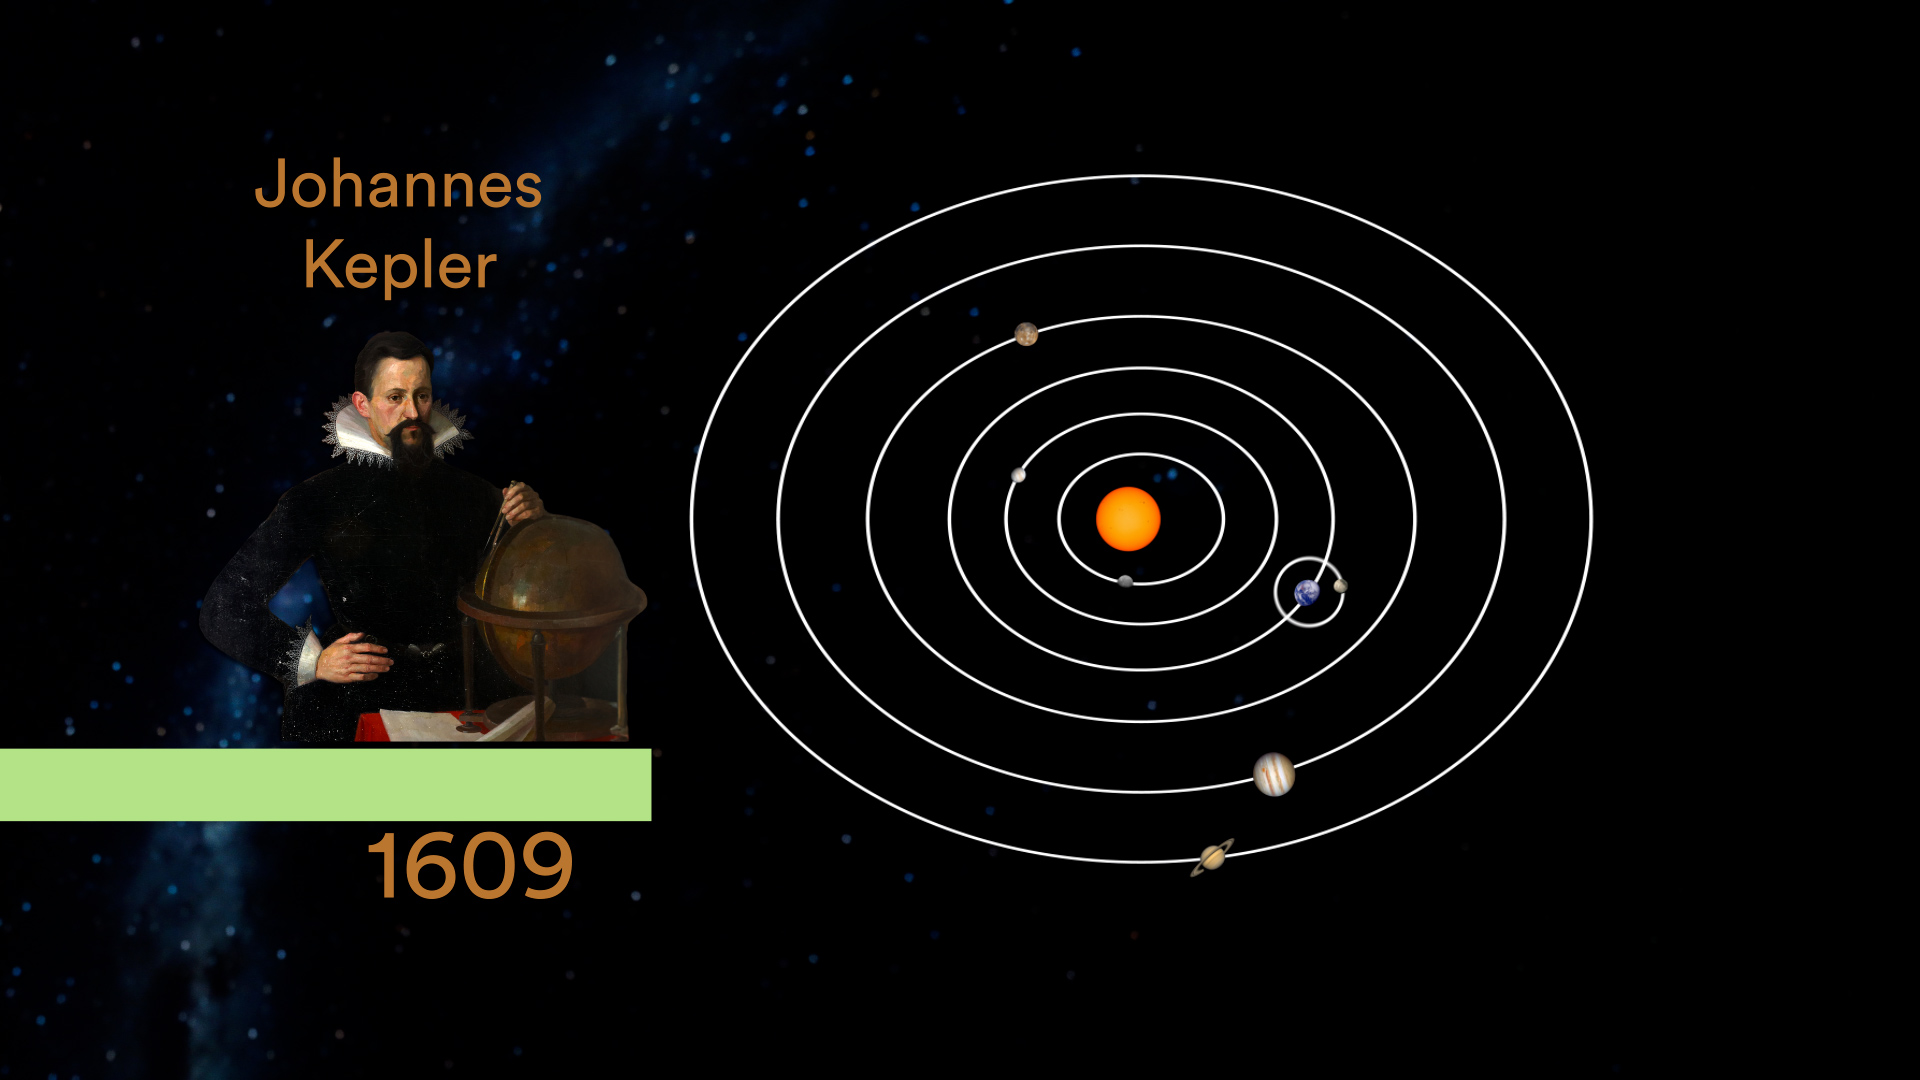
\includegraphics[width=16cm]{ptu-kepler.jpg}
\end{center}
\caption{Kepler's solar system}
\label{kepler1}
\end{figure}
\section{Kepler's Three Laws of Planetary Motion}
In the early 1600s, Johannes Kepler analyzed the precise astronomical observations of Tycho Brahe. He discovered three empirical laws that described planetary motion with remarkable accuracy, moving away from the ancient idea of perfect circular orbits.
\subsection{Kepler's First Law (The Law of Ellipses):}
\begin{quote}
\textit{The orbit of a planet is an ellipse with the Sun at one focus.}
\end{quote}
\begin{itemize}
\item \emph{Key Concept:} An ellipse is an oval shape with two focal points (foci). The Sun is not at the center but at one of these foci. The degree of "oval-ness" is measured by eccentricity (\emph{e}). A circle has e=0; most planetary orbits are nearly circular (e.g., Earth's e \(\approx 0.0167\)).
\end{itemize}
\subsection{Kepler's Second Law (The Law of Equal Areas):}
\begin{quote}
\textit{ A line segment joining a planet and the Sun sweeps out equal areas during equal intervals of time.}
\end{quote}
\begin{itemize}
\item \emph{Key Concept:} A planet moves faster when it is closer to the Sun (perihelion) and slower when it is farther away (aphelion).
The rate at which it "sweeps out area" is constant.
\end{itemize}
\begin{figure}[!ht]
\begin{center}
 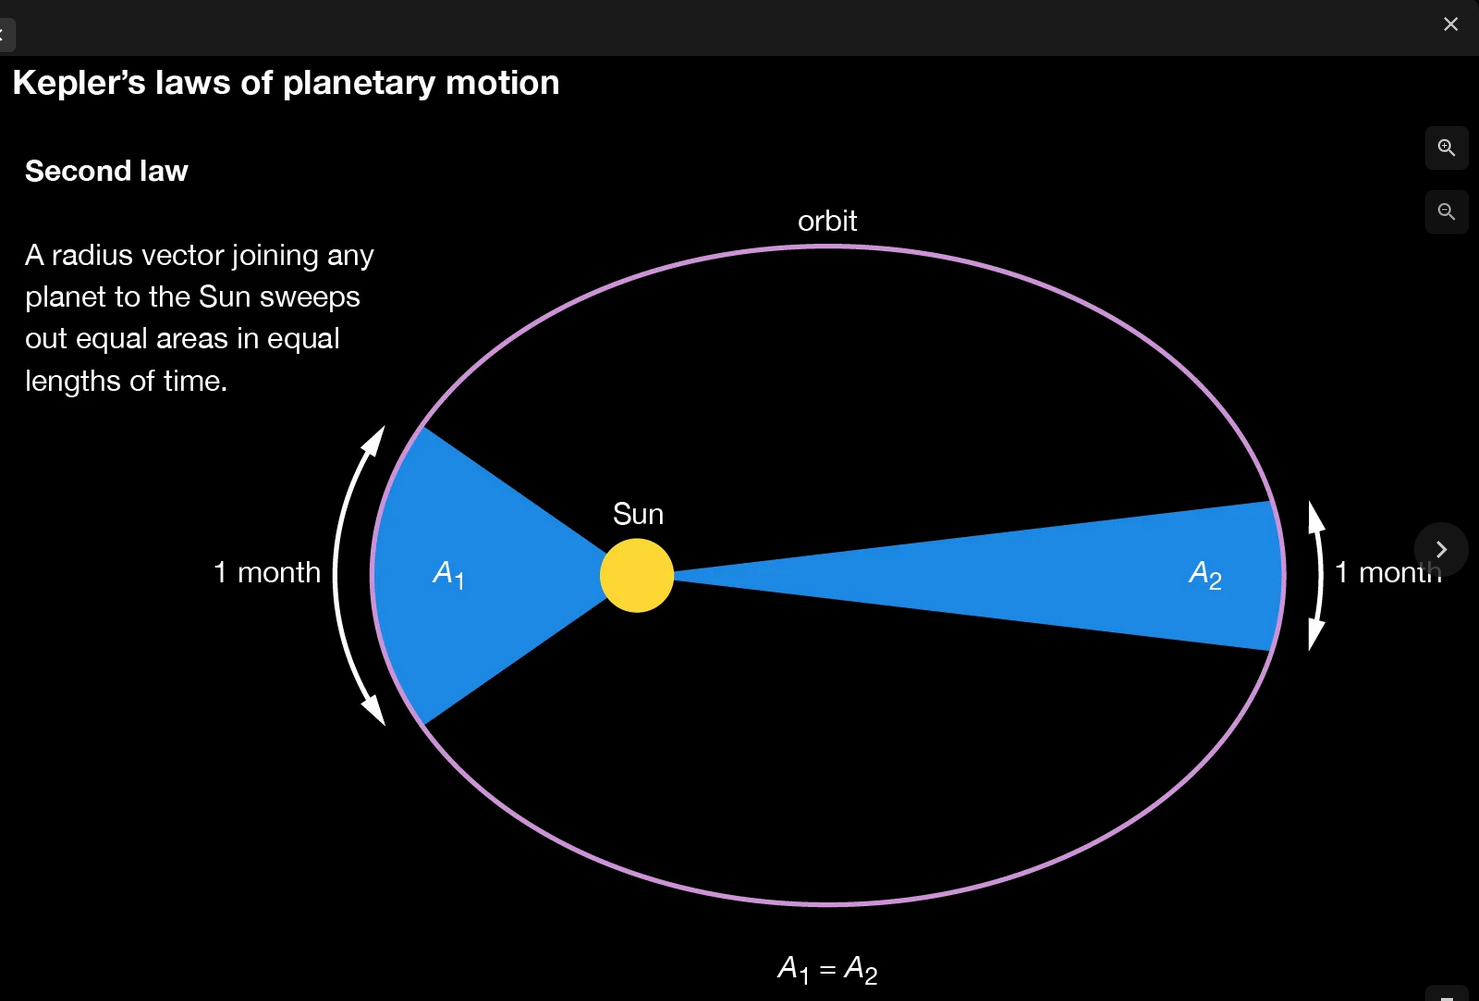
\includegraphics[width=15cm]{Kepler2ndLow.png}
\end{center}
\caption{Kepler 2nd law}
\end{figure}
Kepler’s Second Law, also known as the Law of Equal Areas, describes the speed at which a planet travels as it orbits the Sun. While the First Law defines the \emph{shape} of the orbit (an ellipse), the Second Law explains the \emph{rhythm} of planetary motion.
Kepler’s Second Law (The Law of Equal Areas).\\
In simpler terms, a planet does not move at a constant speed. Its orbital velocity changes depending on how far it is from the Sun.\\
Because orbits are elliptical and the Sun sits at one focus, the distance between the planet and the Sun is constantly changing. To ensure the "area" swept by the imaginary line stays the same, the planet must adjust its speed:
\begin{itemize}
\item At Perihelion (closest to the Sun): The "radius" line is short. To cover a specific area, the planet must travel a longer distance along its orbital path. Therefore, the planet moves at its maximum velocity.
\item At Aphelion (farthest from the Sun): The "radius" line is very long. Only a small movement along the orbit is needed to sweep out the same area. Therefore, the planet moves at its minimum velocity.
\end{itemize}
\begin{table}[h!]
\begin{center}
\begin{tabular}{|c|c|c|}
\hline
\textbf{Position}&\textbf{Distance from Sun}&\textbf{Orbital Speed}\\
\hline
Perihelion&Minimum&Fastest\\
\hline
Aphelion&Maximum&Slowest\\
\hline
\end{tabular}
\end{center}
\end{table}
\emph{The Physics Behind the Law}\\
Kepler derived this law through meticulous observation of planetary data (specifically from Tycho Brahe). However, we now understand that this is a direct consequence of the Conservation of Angular Momentum.
In a system where the only force (gravity) acts along the line connecting the two objects, the angular momentum \emph{L}
remains constant:
\[
 L = m \cdot r \cdot v \cdot \sin(\theta)
\]
Where:
\begin{itemize}
\item  m  is the mass of the planet.
\item  r  is the distance from the Sun.
\item  v  is the orbital velocity.
 \item \(\theta\)  is the angle between the radius vector and the velocity vector.
\end{itemize}
\emph{Historical Significance}\\
This law was revolutionary because it shattered the ancient Greek ideal that celestial bodies must move in "perfect" uniform circles at constant speeds. It provided the empirical groundwork for Isaac Newton to later formulate his Law of Universal Gravitation.
\subsection{Kepler's Third Law (The Harmonic Law):}
\begin{quote}
\textit{The square of the orbital period (\emph{T}) of a planet is directly proportional to the cube of the semi-major axis (\emph{a}) of its orbit.}
\end{quote}
\emph{Formula:} \( T^2 \propto a^3 \) or, more precisely, \( \frac{T^2}{a^3} = \text{constant} \) for all planets orbiting the same central body.\\
While the first two laws describe the motion of a single planet, the Third Law provides a universal rule that links all planets in a system. In simpler terms, as a planet’s distance from the Sun increases, its orbital period (= the time it takes to complete one full revolution) increases significantly.
\begin{itemize}
\item \emph{Key Concept:} This law provides a precise relationship between a planet's distance from the Sun and the time it takes to complete one orbit. The farther a planet is, the longer its year.
\end{itemize}
When expressed using Earth-based units —years for the orbital period (P) and Astronomical Units (AU) for the semi-major axis (a)— the relationship is remarkably simple:
\[
 P^2 = a^3
\]
\begin{table}[h!]
\begin{center}
\begin{tabular}{|c|c|c|c|c|}
\hline
\textbf{Planet}& \textbf{Distance (in AU)}& \textbf{Period (in Earth Years)}& \(P^2\) & \(a^3\)\\
\hline
Mercury&0.39&0.24&\(\sim0.06\)&\(\sim0.06\)\\
\hline
Earth&1.00&1.00&1.00&1.00\\
\hline
Mars&1.52&1.88&\(\sim3.53\)&\(\sim3.51\)\\
\hline
Jupiter&5.20&11.86&\(\sim141\)&\(\sim141\)\\
\hline
\end{tabular}
\end{center}
\end{table}
Note: 1 AU is the average distance from the Earth to the Sun. \\
1 AU = 149597870.700 km\\
\subsubsection{Dynamics: Distance vs. Speed}
The "Harmonic" nature of this law reveals two critical facts about our solar system:
\begin{itemize}
\item Longer Paths: Outer planets have much larger orbits to travel than inner planets.
\item Slower Speeds: Outer planets actually move at slower orbital speeds because the Sun's gravitational pull is weaker at greater distances.
\end{itemize}
This is why Mercury zips around the Sun in just 88 days, while distant Neptune takes about 165 years to complete a single orbit.
\subsubsection{Why is it called the "Harmonic" Law?}
Kepler published this law in 1619 in his work Harmonices Mundi (The Harmony of the World). He believed the universe followed a divine mathematical order similar to musical harmony. He even attempted to express the varying speeds of planets as musical scales, viewing the solar system as a "celestial choir".
\subsubsection{Modern Significance}
Beyond planetary motion, this law is a fundamental tool in modern astronomy:
\begin{itemize}
\item Calculating Mass: It allows scientists to determine the mass of stars, planets, and even the Milky Way Galaxy by observing the orbits of their satellites.
\item Exoplanet Discovery: By measuring the time it takes an exoplanet to orbit its star, astronomers can calculate exactly how far away it is and whether it sits in the "habitable zone".
\item Satellite Placement: It is used to calculate the necessary altitude for artificial satellites, such as geostationary communication satellites, to stay in a fixed position above Earth.
\end{itemize}
\subsection{Example 1: Applying Kepler's Third Law}
\emph{Problem:} Mars has an orbital period of about 1.88 Earth-years. The semi-major axis of Earth's orbit is 1 Astronomical Unit (AU). What is the semi-major axis of Mars' orbit in AU?\\
\emph{Solution:}\\
Using Kepler's Third Law, \( \frac{T^2}{a^3} \) is constant for all planets orbiting the Sun. We can set up a ratio using Earth's values as a reference.\\
For Earth: \( T_{earth} = 1 \, \text{year} \), \( a_{earth} = 1 \, \text{AU} \)\\
For Mars: \( T_{mars} = 1.88 \, \text{years} \), \( a_{mars} = ? \)\\

\[
\frac{T_{earth}^2}{a_{earth}^3} = \frac{T_{mars}^2}{a_{mars}^3}
\]
\[
\frac{1^2}{1^3} = \frac{(1.88)^2}{a_{mars}^3}
\]
\[
1 = \frac{3.5344}{a_{mars}^3}
\]
\[
a_{mars}^3 = 3.5344
\]
\[
a_{mars} = \sqrt[3]{3.5344} \approx 1.52 \, \text{AU}
\]

\emph{Answer:} Mars is, on average, 1.52 times farther from the Sun than Earth is.\\

\section{Newton's Law of Universal Gravitation}

About 50 years after Kepler, Isaac Newton formulated his law of universal gravitation, which explains \emph{why} Kepler's laws work.

\begin{quote}
Every particle in the universe attracts every other particle with a force that is directly proportional to the product of their masses and inversely proportional to the square of the distance between their centers.                                                                                                                                                                                                                      \end{quote}
\emph{Formula:} \( F = G \frac{m_1 m_2}{r^2} \)\\
\begin{itemize}
\item   \emph{F} is the gravitational force (Newtons, N)
\item   \emph{G} is the universal gravitational constant (\( 6.67430 \times 10^{-11} \, \text{N·m}^2/\text{kg}^2 \))
\item   \emph{\(m_1\)} and \(m_2\) are the masses of the two objects (kilograms, kg)
\item   \emph{r} is the distance between their centers (meters, m)
\end{itemize}

\subsection{Example 2: Calculating Gravitational Force}

\emph{Problem:} What is the gravitational force of attraction between the Earth and the Moon?\\
\begin{itemize}
\item   Mass of Earth, \( M_E = 5.97 \times 10^{24} \, \text{kg} \)
\item   Mass of Moon, \( M_M = 7.35 \times 10^{22} \, \text{kg} \)
\item   Average distance between centers, \( r = 3.84 \times 10^8 \, \text{m} \)
\end{itemize}

\emph{Solution:}\\
\[
F = G \frac{M_E M_M}{r^2}
\]
\[
F = (6.67430 \times 10^{-11}) \frac{(5.97 \times 10^{24})(7.35 \times 10^{22})}{(3.84 \times 10^8)^2}
\]
First, calculate the numerator: \( (5.97 \times 10^{24}) \times (7.35 \times 10^{22}) = 4.387 \times 10^{47} \)\\
Then the denominator: \( (3.84 \times 10^8)^2 = 1.475 \times 10^{17} \)\\
Now, \( \frac{4.387 \times 10^{47}}{1.475 \times 10^{17}} = 2.976 \times 10^{30} \)\\
Finally, \( (6.67430 \times 10^{-11}) \times (2.976 \times 10^{30}) \approx 1.98 \times 10^{20} \, \text{N} \)\\
\emph{Answer:} The gravitational force between the Earth and Moon is approximately \( 2.0 \times 10^{20} \, \text{Newtons} \).\\
This immense force is what keeps the Moon in orbit.

\section{How are Explained Kepler's Laws}
Newton showed that his law of gravitation, when combined with his laws of motion, \emph{predicts} Kepler's empirical laws.
\subsection{Explaining Kepler's First Law (Elliptical Orbits):}
Newton demonstrated that the inverse-square nature of the gravitational force (\( F \propto 1/r^2 \)) necessarily leads to \emph{conic sections} as the possible orbits. An ellipse is one type of conic section. The other solutions (like parabolas and hyperbolas) describe the paths of objects that are not gravitationally bound, like some comets.
\subsection{Explaining Kepler's Second Law (Equal Areas):}
This is a consequence of the \emph{conservation of angular momentum}. The gravitational force is a \emph{central force}; it always acts along the line connecting the planet to the Sun. A central force exerts zero torque, meaning angular momentum must be conserved. It can be showed that constant angular momentum is mathematically equivalent to the "equal areas in equal times" rule.\\
The concept of Angular Momentum is fundamentally linked to Kepler’s Second Law, the formal discovery and enunciation of its conservation did not happen all at once. It evolved from a mathematical observation into a core principle of physics.
\subsubsection{The Mathematical Foundation: Leonhard Euler (1744)}
While Johannes Kepler described the behavior of planets (equal areas in equal times), he did not understand the underlying physics. The first person to formally describe the concept of "moment of momentum" (the precursor to angular momentum) was the Swiss mathematician Leonhard Euler.\\
In 1744, Euler began to express the idea that the "quantity of motion" for a rotating body was conserved, specifically in the context of his work on the motion of rigid bodies.
\subsubsection{The Physical Enunciation: Daniel Bernoulli (1744)}
In the same year, Daniel Bernoulli (a contemporary and friend of Euler) stated the principle more clearly in a physical sense. He realized that for a system not subject to an external torque, the total moment of momentum remains constant.
Bernoulli and Euler essentially "discovered" the principle while trying to apply Newton’s laws of motion to rotating objects—something Newton himself hadn't fully explored in his Principia.
\subsubsection{The "Law of Areas": Patrick d'Arcy (1747)}
The specific connection between Kepler’s Second Law and the conservation of angular momentum was formalized by the Irish-born mathematician Patrick d'Arcy.
\begin{itemize}
\item In 1747, he published his "Principle of Areas."
\item He explicitly stated that for any system of bodies acting on each other (under central forces), the sum of the products of the masses and the areas described by their radius vectors remains constant.
\item This was the definitive proof that Kepler's Second Law was actually the Conservation of Angular Momentum in action.
\end{itemize}
\begin{table}[h!]
\begin{center}
\begin{tabular}{|c|c|c|}
\hline
\textbf{Scientist}&\textbf{Contribution}&\textbf{Year}\\
\hline
Johannes Kepler&Observed the result (Equal Areas Law) but lacked the physics.&1609\\
\hline
Leonhard Euler&Developed the mathematical "moment of momentum."&1744\\
\hline
Patrick d'Arcy&Enunciated the "Law of Areas" as a conservation principle.&1747\\
\hline
Emmy Noether&Proved why it's conserved (due to rotational symmetry).& 1915\\
\hline
\end{tabular}
\end{center}
\caption{Key Milestone Summary}
\end{table}
\subsubsection{The "Deep" Why: Noether’s Theorem}
It is worth noting that we didn't fully understand why angular momentum is conserved until Emmy Noether published her famous theorem in 1915. She proved that every conservation law is tied to a symmetry in nature:
\begin{quote}
    \emph{Angular Momentum is conserved because space is isotropic} (it has no preferred direction).
\end{quote}
If you rotate an entire physics experiment by \(90^{\circ}\), the laws of physics don't change—and that "symmetry" is what forces angular momentum to stay constant
\subsection{Deriving Kepler's Third Law (from Newton's Law):}
This is the most powerful connection. Let's derive it for a circular orbit (a special case of an ellipse where the semi-major axis 'a' is the radius 'r').
For a planet of mass \( m \) orbiting the Sun of mass \( M_S \) at a distance \( r \), two things are true:
\begin{enumerate}
\item \emph{Newton's 2nd Law:} The gravitational force provides the centripetal force: \( G \frac{M_S m}{r^2} = m a_c \)
\item \emph{Centripetal Acceleration:} \( a_c = \frac{v^2}{r} \)
\end{enumerate}
Substituting (2) into (1):\\
\[
G \frac{M_S m}{r^2} = m \frac{v^2}{r}
\]
Cancel \( m \) and one \( r \):
\[
G \frac{M_S}{r} = v^2
\]
The orbital velocity \( v \) is the circumference (\( 2\pi r \)) divided by the period (\( T \)): \( v = \frac{2\pi r}{T} \)\\
Substitute for \( v^2 \):\\
\[
G \frac{M_S}{r} = \left( \frac{2\pi r}{T} \right)^2
\]
\[
G \frac{M_S}{r} = \frac{4\pi^2 r^2}{T^2}
\]
Now, rearrange to get \( T^2 \) on one side:\\
\[
T^2 = \frac{4\pi^2 r^2}{G M_S} \cdot r
\]
\[
T^2 = \left( \frac{4\pi^2}{G M_S} \right) r^3
\]
Since for an ellipse, we use the semi-major axis \( a \), the general form is:
\[
\boxed{T^2 = \frac{4\pi^2}{G M_S} a^3}
\]
This is Kepler's Third Law! Notice that \( \frac{4\pi^2}{G M_S} \) is a \emph{constant} because G and the mass of the Sun are constant. Therefore, \( T^2 \propto a^3 \), exactly as Kepler stated.

\section{Summary}
\begin{itemize}
\item   \emph{Kepler} described \emph{how} the planets move (kinematics).
\item   \emph{Newton} explained \emph{why} they move that way by providing the underlying force (dynamics).
\item   \emph{Newton}'s Law of Universal Gravitation is the fundamental principle that, when applied, mathematically predicts and validates the Kepler's Laws.
\end{itemize}
This elegant connection between observation and theory is a cornerstone of classical physics and our understanding of the cosmos.
\section{Satellites in Space}
To understand how we control things in space—from the Hubble Space Telescope to a simple communication satellite—we have to look at how we manage rotation (attitude) using the Conservation of Angular Momentum.
When a satellite points a telescope at a star, it uses a \emph{Control Loop}:
\begin{enumerate}
\item \emph{Sense}: A Star Tracker takes a photo of the sky and compares it to a map to find the current quaternion
\(q_{current}\).
\item \emph{Calculate}: The computer finds the difference between the target \(q_{target}\) and \(q_{current}\).
\item \emph{Actuate}: The computer commands the Reaction Wheels to change speed.
\item \emph{Stabilize}: If external forces (like solar radiation pressure) add unwanted momentum, the satellite uses Magnetorquers (electromagnets that push against Earth's magnetic field) to "dump" the excess momentum.
\end{enumerate}
\subsection{The Physics: Gyroscopes and Reaction Wheels}
In space, there is no air to push against. To rotate, a satellite uses Reaction Wheels (high-speed flywheels).
\begin{itemize}
\item \textbf{The Principle}: If a satellite is at rest and starts spinning an internal wheel clockwise, the satellite body must rotate counter-clockwise to keep the total angular momentum L at zero.
\item \textbf{The Math}:
\[
 \Delta L_{wheel} +  \Delta L_{satellite} = 0
\]
If the wheel has a moment of inertia \(I_w\) and spins at velocity \(\omega_w\), and the satellite has a moment of inertia \(I_s\) and rotates at \(\omega_s\):
\end{itemize}
Example Computation:\\
If a satellite ( \(I_s = 500\,kg \cdot m^2 \) ) wants to rotate at 0.1 rad/s and uses a reaction wheel (\(I_w = 0.05\,kg \cdot m^2\)), how fast must the wheel spin?
\[
 \omega_w = \frac{500 \cdot 0.1}{0.05} = 1000\, rad/s \approx 9550\,RPM
\]
\subsection{Expressing Rotations: Euler Angles vs. Quaternions}
To point a satellite instrument (like a camera), we need a mathematical way to describe its orientation in 3D space.
\subsubsection{\emph{Euler Angles} (The Intuitive Way)}
Euler angles describe a rotation as three successive turns around specific axes (e.g., Roll, Pitch, and Yaw -in italian Rollio, beccheggio e imbardata-).\\
To be more clear, we can imagine a plane\\
Rotations:
\begin{itemize}
\item roll (rollio), around the longitudinal X axis, also called the rolling axis (One wing of the plane up, the other wing down)
\item pitch (beccheggio), around the transverse Y axis, also called the lateral or pitch axis (the head of the plane up or down)
\item yaw (imbardata), around the vertical Z axis, also called the yaw axis (the head of the plane left or right)
\end{itemize}
\begin{itemize}
\item Pros: Easy for humans to visualize.
\item Cons: Gimbal Lock (blocco cardanico in italian). If two axes align (e.g., a \(90^{\circ}\)pitch), you lose one degree of freedom, and the math "breaks" (singularities). From the gyroscope formulations it is possible to derive the matrix equations of the auxiliary kinematic relations of attitude. Using Euler angles they have the following form:\\
\[
\begin{bmatrix}
\dot{x}\\
\dot{y}\\
\dot{z}\\
\end{bmatrix}
=
\begin{bmatrix}
1 & \frac{\sin(\phi)\sin(\theta)}{\cos(\theta)}& \frac{\cos(\phi)\sin(\theta)}{\cos(\theta)}\\
0 & \cos(\phi)& -\sin(\phi)\\
0 & \frac{\sin(\phi)}{\cos(\theta)}& \frac{\cos(\phi)}{\cos(\theta)} \\
\end{bmatrix}
\begin{bmatrix}
\dot{p}\\
\dot{q}\\
\dot{r}\\
\end{bmatrix}
\]
The matrix presents obvious singularities when the denominators are zero, that is, when \({\displaystyle \theta =\pm {\frac {\pi }{2}}}\).
\end{itemize}
The \emph{Kinematic Differential Equation of attitude} maps the angular velocities measured by the satellite's internal sensors to the rate of change of the satellite's orientation in space.
\begin{itemize}
\item The Vector \([ \dot{x}\,\, \dot{y}\,\, \dot{z} ]^T\) (Euler Angle Rates)\\
These are the time derivatives of the Euler Angles. While your source uses x,y,z, they almost always represent the standard aeronautical angles:
\begin{itemize}
\item \(\dot{x} = \dot{\phi} \) {\small (Roll rate): The rate of rotation around the longitudinal axis.}
\item \(\dot{y} = \dot{\theta} \) (Pitch rate): The rate of rotation around the lateral axis.
\item \(\dot{z} = \dot{\psi} \) (Yaw rate): The rate of rotation around the vertical axis.
\end{itemize}
\item The Vector \([ \dot{p}\,\, \dot{q}\,\, \dot{r} ]^T\) (Body Angular Velocities)\\
These are the Body-Fixed Angular Velocities. These are the raw values provided by the Gyroscopes.
\end{itemize}
Important Notes:\\
\begin{itemize}
\item It's written \(\dot{p}\,\, \dot{q}\,\, \dot{r}\), but in standard kinematics, these are just p,q,r. They are already "rates" (radians per second). Using a "dot" over them would imply angular acceleration (the derivative of the gyro reading).
\item p: Rotation rate about the satellite's own X-axis.
\item q: Rotation rate about the satellite's own Y-axis.
\item e: Rotation rate about the satellite's own Z-axis.
\end{itemize}
\begin{figure}[!ht]
\begin{center}
 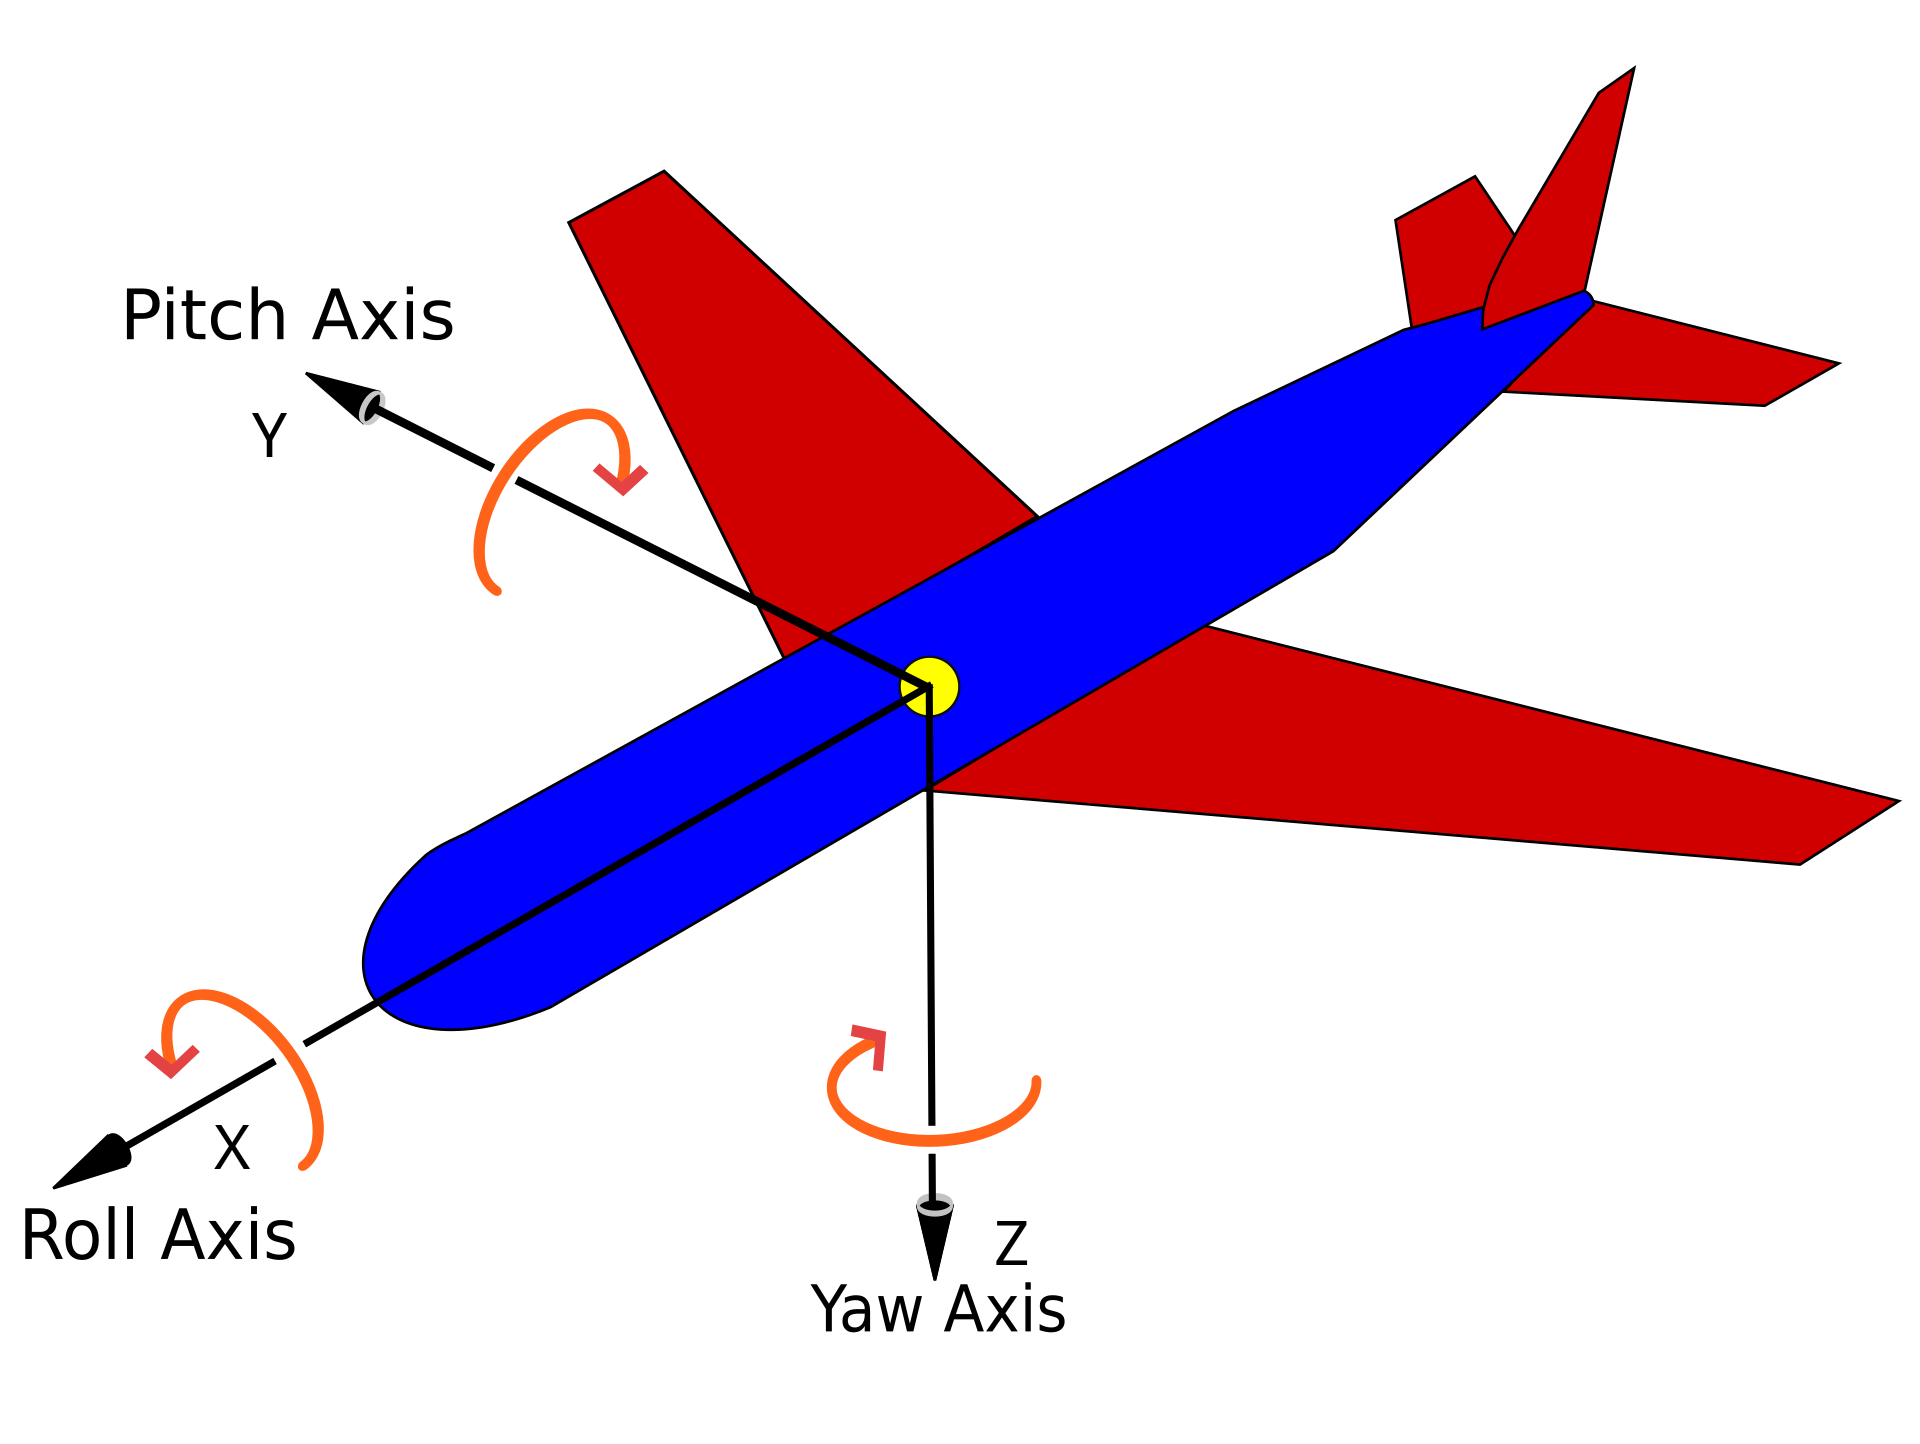
\includegraphics[width=15cm]{Yaw_Axis_Corrected001.png}
\end{center}
\caption{Roll, Pitch and Yaw angles}
\end{figure}
\subsubsection{Why is the Matrix Necessary?}
You might wonder: "Why can't we just say \(\dot{\phi} = p \)?"\\
The reason is that p, q, r are measured in the \emph{Body Frame} (which is spinning with the satellite), while
\( \phi,\, \theta,\, \psi\) are measured relative to a fixed \emph{Inertial Frame} (like the stars).\\
As the satellite rotates, the axes of the gyroscopes tilt. The matrix (the Direction Cosine Matrix derivative) "un-tilts" those measurements to tell you how the Euler angles are changing relative to the fixed universe.
\subsubsection{The Singularity: Gimbal Lock}
The terms involving \( \frac{1}{\cos(\theta)}\) (or \(\sec(\theta)\) ) become undefined when
\(\theta = \pm 90^{\circ}\) (\(\pm \pi/2\) ).
\begin{itemize}
\item \emph{Mathematical reason}: \( \cos(90^{\circ}) = 0\), leading to a division by zero.
\item \emph{Physical reason}: At a \(90^{\circ}\) pitch, the Roll axis and the Yaw axis become perfectly aligned. The system "loses" one degree of freedom because it can no longer distinguish between a roll and a yaw.
\end{itemize}
\subsubsection{How to Correct "Wobbling" Data}
Using this knowledge to correct images affected by wobbling:
\begin{itemize}
\item \textbf{Integration}: You take the gyro readings (p, q, r), plug them into that matrix, and integrate over time to find the current Euler angles (\(\phi, \theta,\psi\)).
\item \textbf{The "Correction" Matrix}: Once you have the angles, you build a \textbf{Rotation Matrix} \( R(\phi,\theta,\psi) \).
\item \textbf{Pixel Transformation}: For every pixel in your "wobbled" image, you multiply its coordinates by the inverse of that rotation matrix \( R^{-1} \) to find where that pixel should have landed on a stable map.
\end{itemize}
\[  P_{corrected} = R(\phi,\theta,\psi)^{-1} \cdot P_{distorted} \]
The components (\(\dot{x}\,\, \dot{y}\,\, \dot{z}\)) represent the Euler angle rates (\( \phi,\, \theta,\, \psi\)), which describe how the satellite's orientation changes relative to the stars. The components are the body-fixed angular velocities measured directly by the gyroscopes. The matrix acts as a bridge to convert local sensor data into global orientation changes, but it fails at \( \theta = \pm90^{\circ}\) due to Gimbal Lock.
\subsubsection{\emph{Quaternions} (The Computer's Way)}
Quaternions represent a rotation as a single vector (the axis of rotation) and a scalar (the amount of rotation). A quaternion q is written as:
\[
 q = w + xi + yj + zk
\]
where \( w^2 + z^2 + y^2 + z^2 = 1 \) (unit quaternion).
\begin{table}[h!]
\begin{center}
\begin{tabular}{|c|c|c|}
\hline
\textbf{Feature}&\textbf{Euler Angles}&\textbf{Quaternions} \\
\hline
Intuition&High (Roll, Pitch, Yaw)&Low (4D complex numbers) \\
\hline
Computation&Heavy (Trigonometry)&Fast (Algebraic) \\
\hline
Singularities&Yes (Gimbal Lock)&No \\
\hline
Animation/Interpolation&Jerky&Smooth (SLERP) \\
\hline
\end{tabular}
\end{center}
\caption{Comparison Table}
\end{table}
\subsection{Computation Example: Quaternions}
If you want to rotate a satellite by an angle \( \theta \) around a unit vector axis \(\vec{u} = (u_x,u_y,u_z) \)
, the quaternion is:
\[
 q = [\cos \begin{pmatrix}\frac{\theta}{2}\end{pmatrix},u_x\sin \begin{pmatrix}\frac{\theta}{2} \end{pmatrix},u_y\sin \begin{pmatrix}\frac{\theta}{2}\end{pmatrix},u_z\sin \begin{pmatrix} \frac{\theta}{2}\end{pmatrix}]
\]
\textbf{Task}: Rotate \( 90^{\circ}\)(1.57 rad) around the Z-axis (0,0,1).
\begin{itemize}
\item \(\cos(45^{\circ})\) = 0.707
\item \(\sin(45^{\circ})\) = 0.707
\item \(q = [0.707, 0, 0, 0.707]\)
\end{itemize}
This 4-element vector is what the satellite's flight software uses to adjust the speed of the reaction wheels with zero risk of mathematical errors or "Gimbal Lock".
In current space missions quaternions are the standard because they provide a global, non-singular representation of attitude, entirely avoiding the gimbal lock seen in Euler angles.
\subsubsection{The Quaternion Kinematic Equation}
To resolve the singularity at \( \theta = \pm 90^{\circ}\), we replace the Euler angle rates with the quaternion rate of change (\(\dot{q}\)). The relationship between the satellite's body angular velocity \( \vec{\omega} = [ p\,\, q\,\, r ]^T \) (measured by gyroscopes) and the time derivative of the attitude quaternion q is expressed by the following matrix equation:
\[
\begin{bmatrix}
\dot{q_1}\\
\dot{q_2}\\
\dot{q_3}\\
\dot{q_4}\\
\end{bmatrix}
= \frac{1}{2}
\begin{bmatrix}
0&r&-q&p\\
-r&0&p&q\\
q&-p&0&r\\
-p&-q&-r&0\\
\end{bmatrix}
\begin{bmatrix}
q_1\\
q_2\\
q_3\\
q_4\\
\end{bmatrix}
\]
Alternatively, this is often written in a compact form as a quaternion product:
\[
 \dot{q}=\frac{1}{2}q \otimes \omega_{body}
\]
where \(  \omega_{body} \) is treated as a "pure" quaternion with a scalar part of zero: \([p,q,r,0]^{T}\).
\subsubsection{Why Quaternions Solve the "Singularity" Problem}
\begin{itemize}
\item \emph{No Division by Zero}: Unlike the Euler matrix, which contains \( \frac{1}{\cos(\theta)}\), the quaternion kinematic matrix contains only the raw components of p, q, r. There are no trigonometric denominators that can vanish.
\item \emph{Four-Dimensional Coverage}: Quaternions use four parameters to describe three degrees of freedom. This "over-defined" representation ensures every possible orientation is uniquely and smoothly represented, even when axes align.
\item \emph{Computational Efficiency}: Integrating \( \dot{q} \) involves simple linear algebra (multiplication and addition), making it significantly faster for onboard computers than the heavy trigonometry required for Euler angles.
\end{itemize}
\subsubsection{Application: Correcting "Wobbled" Measurements}
For planetary missions like BepiColombo, where precise instrument pointing is critical despite potential spacecraft nutation (wobble), the process of correcting acquired measurements follows these steps:
\begin{enumerate}
\item \emph{High-Frequency Integration}: The onboard computer (or ground processing) takes high-rate gyro data (p, q, r) and integrates the \( \dot{q} \) equation above.\\
\textit{Note}: Because of numerical drift, the resulting q must be constantly re-normalized to unit length (|q| = 1) to remain a valid rotation.
\item \emph{Attitude Reconstruction}: For any specific measurement time t (e.g., a pixel captured by a camera), a precise quaternion q(t) is calculated by interpolating between the known state vectors.
\item \emph{Coordinate Transformation}: To correct a sensor measurement \( \vec{v}_{body}\) and place it accurately on a map (Inertial or Planetary frame), the following rotation is applied:
\[
\vec{v}_{inertial} = q \otimes \vec{v}_{body} \otimes q^{-1}
\]

If the satellite is "spinning" or "wobbling", q changes rapidly, but because the kinematics are non-singular, the transformation remains stable and accurate across all orientations.
\subsubsection{Special Considerations for Space Missions}
\begin{itemize}
\item \emph{The Unwinding Phenomenon}: One unique challenge with quaternions is that q and -q represent the same physical attitude. If a control system isn't carefully designed, it might attempt to rotate the spacecraft \(360^{\circ}\) "the long way around" to reach a target orientation—an effect known as unwinding.
\item \emph{Scalar Order}: In your work with ESA and ASI, it is vital to check the convention used. Some systems place the scalar component first (\( q = [ w,\,x,\,y,\,z] \)), while others place it last ( \( q = [x,\,y,\,z,\,w] \)). This changes the structure of the kinematic matrix.
\end{itemize}
\end{enumerate}
\subsection{Other examples}
To correct measurements from a moving satellite, we must bridge the gap between the
Sensor Frame (what the camera sees) and the Inertial Frame (the actual sky or ground map). When a satellite wobbles or spins, the "bridge" between these frames changes every millisecond.
\subsubsection{Gimbal Lock}
Gimbal lock is why we use Quaternions instead of Euler Angles (\emph{roll, pitch, yaw}) for stabilization.
Imagine three nested rings (gimbals).\\
\begin{itemize}
\item Normal State: The three axes are orthogonal (\(90^{\circ}\) to each other). You can move in any direction.
\item Locked State: If you rotate the middle ring by \(90^{\circ}\), the inner ring and outer ring become aligned in the same plane.
\end{itemize}
\begin{verbatim}
       [ Pitch ]              [ Pitch & Yaw Aligned ]
         |                          ||
 [Roll]--o--[Yaw]       =>          o--[Roll]
         |                          ||
   (3 Degrees of Freedom)     (Lost 1 Degree of Freedom)
\end{verbatim}
In this state, the math behind Euler angles encounters a \emph{division by zero}. The satellite "doesn't know" how to calculate a turn in the lost dimension, leading to a loss of control. \emph{Quaternions} avoid this by calculating the rotation as a single arc on a 4D sphere.
\subsubsection{Star Tracker Identification}
The "Lost-in-Space" Algorithm. A Star Tracker is a camera that looks at the stars to find the satellite's orientation.
\emph{The Process}:
\begin{enumerate}
\item \emph{Centroiding}: The camera takes a blurry photo of stars. It calculates the center of brightness for each star (x,y coordinates on the sensor).
\item \emph{Pattern Matching (The "Triangle" Method)}: The computer selects the brightest stars and measures the angular distances between them.
\item \emph{Database Comparison}: It compares these "triangles" to a star catalog (like the Hipparcos catalog).
\end{enumerate}
\emph{Visualizing the Match}
\begin{verbatim}
Sensor Image:             Star Catalog Map:
   * (A)                     * (Alpha)
    \                         \
     \                         \
      * (B)-------* (C)         * (Beta)-------* (Gamma)

Result: Triangle ABC matches Alpha-Beta-Gamma.
The algorithm now knows exactly where the camera is pointing.
\end{verbatim}
\subsubsection{Correcting Measurements}
The "De-Wobbling" Math. If a satellite is spinning or wobbling (nutation), an image will be smeared or distorted. To "rectify" the image, we use \emph{Attitude Data Reconstruction}.\\
\emph{The Coordinate Transformation}\\
To map a pixel (u,v) from your camera to a coordinate (Lat, Lon) on a planet or (RA, Dec) in the sky, you apply a rotation matrix R:
\[
 \vec{P}_{Inertial} = [R_{Attitude}] \cdot  [R_{Alignment}] \cdot \vec{P}_{Sensor}
\]
\begin{itemize}
\item \([R_{Alignment}]\): Corrects for the fact that the camera might be slightly crooked on the satellite bus.
\item \([R_{Attitude}]\): This is the \emph{time-varying} matrix derived from your Star Tracker or Gyroscopes.
\end{itemize}
\emph{Correcting Spin (Image Rectification)}
If the satellite is spinning, a "Push-broom" sensor (like those on many Earth-observation satellites) acquires one line of pixels at a time. If the satellite wobbles, the lines won't be parallel; they will look like a "zigzag."
\emph{How to fix it}:\\
\begin{enumerate}
\item Timestamping: Every line of pixels is assigned a high-precision GPS timestamp.
\item Attitude Interpolation: We look at the gyroscope data at that exact timestamp. Since gyros sample faster than cameras, we interpolate between two readings to find the exact quaternion.
\item Re-sampling: We "shift" the pixels back to where they should have been if the satellite were stable
\end{enumerate}
\begin{table}[h!]
\begin{center}
\begin{tabular}{|c|c|c|}
\hline
\textbf{Measurement Type}&\textbf{Effect of Wobble}&\textbf{Correction Method}\\
\hline
\emph{Point Source (Stars)}&"Star Trails" or Blur & {\tiny Deconvolution using the known "Point Spread Function" of the wobble.}\\
\hline
\emph{Planetary Mapping}&Geometric Distortion & {\tiny Orthorectification (re-projecting pixels onto a digital elevation model).}\\
\hline
\emph{Multi-band Images}&Bands don't overlap & {\tiny Co-registration (aligning the Blue band to the Red band using the time-offset).}\\
\hline
\end{tabular}
\end{center}
\caption{Correcting Satellite Data}
\end{table}
\subsubsection{Example Computation: Correcting a Pixel}
Imagine your satellite has a small yaw wobble of \( \Delta \varPsi = 0.01^{\circ} \) at the moment an image is taken. Your focal length is \( f = 1000\,mm \).\\
The displacement on the sensor \( ( \Delta d ) \) is:
\[ \Delta d = f \cdot \tan(\Delta \varPsi) \]
\[ \Delta d = 1000 \cdot \tan(0.01^{\circ} \approx 0.174\,mm) \]
If your pixels are 10 microns (0.01 mm ), that wobble caused a shift of 17 pixels. To correct the data, the software must move that line of pixels 17 positions back in the opposite direction before saving the final map.
\subsection{Visualization}
To visualize the complex geometry of satellite attitude and image reconstruction, you can use specialized online interactive tools or generate your own visualizations using languages like Python, C or Java and dedicated software libraries.
\subsubsection{Recommended Online Visual Sources}
The following sources provide interactive animations that are much clearer than static images for understanding rotations:
\begin{itemize}
\item \emph{Gimbal Lock \& Euler Angles}: The Yaw/Pitch/Roll Gimbal Visualization allows you to manipulate rings and see exactly when they align to cause a loss of a degree of freedom.
\item \emph{Quaternion Interaction}: For a deep dive into how Quaternions avoid these issues, Ben Eater’s Explorable Video Series provides an interactive 4D-to-3D projection.
\item \emph{Star Maps \& Data Sets}: The NASA Scientific Visualization Studio offers high-resolution deep star maps used in satellite animation and star tracker testing.
\item \emph{Planetary Mapping Tools}: The USGS Map a Planet (MAP) and PILOT (Planetary Image Locator Tool) are cloud processing tools that allow you to see how raw planetary images are map-projected and orthorectified.
\end{itemize}
\subsubsection{Python Script for Attitude Visualization}
The following script uses matplotlib to demonstrate how a satellite's boresight (where its camera points) moves in 3D space when affected by a "wobble." It shows the difference between a stable pointing and a disturbed one.
{
\scriptsize
\begin{verbatim}
import numpy as np
import matplotlib.pyplot as plt
from mpl_toolkits.mplot3d import Axes3D

def rotate_vector(v, angle_deg, axis):
    """Simple rotation of a vector around X, Y, or Z axis."""
    rad = np.radians(angle_deg)
    if axis == 'x':
        R = np.array([[1, 0, 0], [0, np.cos(rad), -np.sin(rad)], [0, np.sin(rad), np.cos(rad)]])
    elif axis == 'y':
        R = np.array([[np.cos(rad), 0, np.sin(rad)], [0, 1, 0], [-np.sin(rad), 0, np.cos(rad)]])
    else: # z
        R = np.array([[np.cos(rad), -np.sin(rad), 0], [np.sin(rad), np.cos(rad), 0], [0, 0, 1]])
    return R.dot(v)

# 1. Define original camera boresight (pointing along Z axis)
boresight = np.array([0, 0, 1])

# 2. Simulate a wobble (Nutation)
time = np.linspace(0, 10, 100)
wobble_x = 5 * np.sin(time) # 5 degree wobble in pitch
wobble_y = 5 * np.cos(time) # 5 degree wobble in yaw

points = []
for i in range(len(time)):
    v = rotate_vector(boresight, wobble_x[i], 'x')
    v = rotate_vector(v, wobble_y[i], 'y')
    points.append(v)

points = np.array(points)

# 3. Plotting
fig = plt.figure(figsize=(10, 7))
ax = fig.add_subplot(111, projection='3d')

# Plot the "Target" center
ax.quiver(0, 0, 0, 0, 0, 1, color='green', label='Ideal Pointing', length=1.2)

# Plot the "Wobbling" path
ax.plot(points[:,0], points[:,1], points[:,2], color='red', label='Satellite Wobble Path')
ax.scatter(points[-1,0], points[-1,1], points[-1,2], color='red')

ax.set_title("Satellite Boresight Wobble (Attitude Error)")
ax.set_xlim([-1, 1]); ax.set_ylim([-1, 1]); ax.set_zlim([0, 1.5])
ax.legend()
plt.show()
\end{verbatim}
}
\subsubsection{How to use this for Correction}
To "correct" your acquired measurements:
\begin{enumerate}
\item \emph{Inverse Rotation}: Use the inverse of the rotation matrix (or the conjugate of the quaternion) calculated from your star tracker at each timestamp t.
\item \emph{Pixel Mapping}: In Python, you can use SciPy's map\_coordinates to "pull" the pixels from the wobbled locations back into a stable grid.
\item \emph{Advanced Tools}: For professional planetary mapping, you can use the ISIS (Integrated Software for Imagers and Spectrometers) software package, which is the standard used by NASA for manipulating planetary mission imagery.
\end{enumerate}
\begin{figure}[!ht]
\begin{center}
 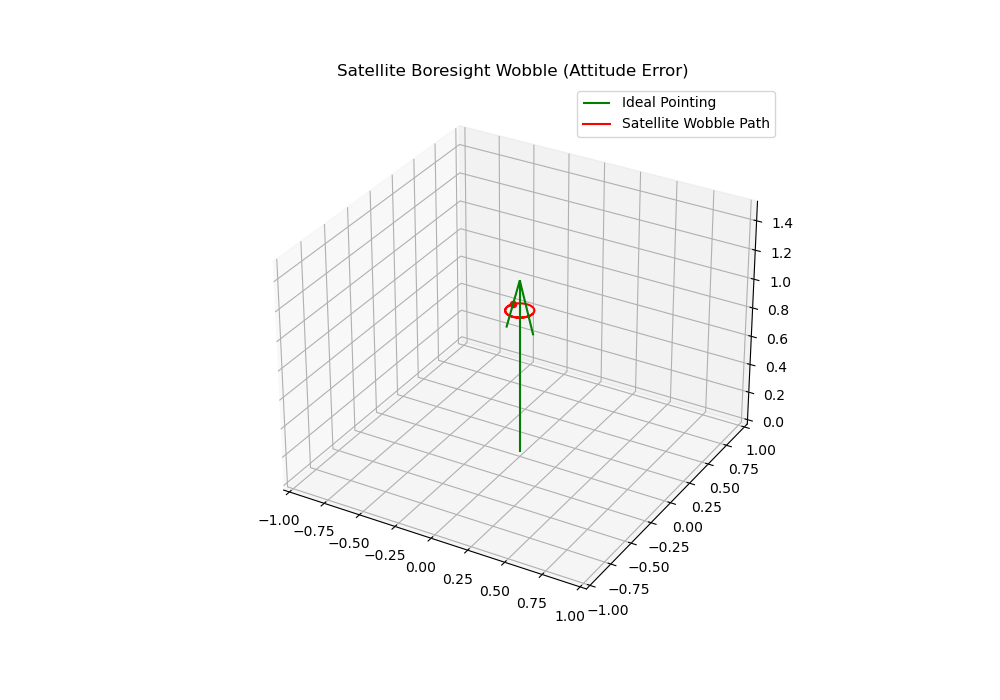
\includegraphics[width=15cm]{satdrift_1.png}
\end{center}
\caption{Correcting satellite drift}
\end{figure}

\end{document}
